\documentclass[twoside]{book}

% Packages required by doxygen
\usepackage{fixltx2e}
\usepackage{calc}
\usepackage{doxygen}
\usepackage[export]{adjustbox} % also loads graphicx
\usepackage{graphicx}
\usepackage[utf8]{inputenc}
\usepackage{makeidx}
\usepackage{multicol}
\usepackage{multirow}
\PassOptionsToPackage{warn}{textcomp}
\usepackage{textcomp}
\usepackage[nointegrals]{wasysym}
\usepackage[table]{xcolor}

% Font selection
\usepackage[T1]{fontenc}
\usepackage[scaled=.90]{helvet}
\usepackage{courier}
\usepackage{amssymb}
\usepackage{sectsty}
\renewcommand{\familydefault}{\sfdefault}
\allsectionsfont{%
  \fontseries{bc}\selectfont%
  \color{darkgray}%
}
\renewcommand{\DoxyLabelFont}{%
  \fontseries{bc}\selectfont%
  \color{darkgray}%
}
\newcommand{\+}{\discretionary{\mbox{\scriptsize$\hookleftarrow$}}{}{}}

% Page & text layout
\usepackage{geometry}
\geometry{%
  a4paper,%
  top=2.5cm,%
  bottom=2.5cm,%
  left=2.5cm,%
  right=2.5cm%
}
\tolerance=750
\hfuzz=15pt
\hbadness=750
\setlength{\emergencystretch}{15pt}
\setlength{\parindent}{0cm}
\setlength{\parskip}{3ex plus 2ex minus 2ex}
\makeatletter
\renewcommand{\paragraph}{%
  \@startsection{paragraph}{4}{0ex}{-1.0ex}{1.0ex}{%
    \normalfont\normalsize\bfseries\SS@parafont%
  }%
}
\renewcommand{\subparagraph}{%
  \@startsection{subparagraph}{5}{0ex}{-1.0ex}{1.0ex}{%
    \normalfont\normalsize\bfseries\SS@subparafont%
  }%
}
\makeatother

% Headers & footers
\usepackage{fancyhdr}
\pagestyle{fancyplain}
\fancyhead[LE]{\fancyplain{}{\bfseries\thepage}}
\fancyhead[CE]{\fancyplain{}{}}
\fancyhead[RE]{\fancyplain{}{\bfseries\leftmark}}
\fancyhead[LO]{\fancyplain{}{\bfseries\rightmark}}
\fancyhead[CO]{\fancyplain{}{}}
\fancyhead[RO]{\fancyplain{}{\bfseries\thepage}}
\fancyfoot[LE]{\fancyplain{}{}}
\fancyfoot[CE]{\fancyplain{}{}}
\fancyfoot[RE]{\fancyplain{}{\bfseries\scriptsize Generated by Doxygen }}
\fancyfoot[LO]{\fancyplain{}{\bfseries\scriptsize Generated by Doxygen }}
\fancyfoot[CO]{\fancyplain{}{}}
\fancyfoot[RO]{\fancyplain{}{}}
\renewcommand{\footrulewidth}{0.4pt}
\renewcommand{\chaptermark}[1]{%
  \markboth{#1}{}%
}
\renewcommand{\sectionmark}[1]{%
  \markright{\thesection\ #1}%
}

% Indices & bibliography
\usepackage{natbib}
\usepackage[titles]{tocloft}
\setcounter{tocdepth}{3}
\setcounter{secnumdepth}{5}
\makeindex

% Hyperlinks (required, but should be loaded last)
\usepackage{ifpdf}
\ifpdf
  \usepackage[pdftex,pagebackref=true]{hyperref}
\else
  \usepackage[ps2pdf,pagebackref=true]{hyperref}
\fi
\hypersetup{%
  colorlinks=true,%
  linkcolor=blue,%
  citecolor=blue,%
  unicode%
}

% Custom commands
\newcommand{\clearemptydoublepage}{%
  \newpage{\pagestyle{empty}\cleardoublepage}%
}

\usepackage{caption}
\captionsetup{labelsep=space,justification=centering,font={bf},singlelinecheck=off,skip=4pt,position=top}

%===== C O N T E N T S =====

\begin{document}

% Titlepage & ToC
\hypersetup{pageanchor=false,
             bookmarksnumbered=true,
             pdfencoding=unicode
            }
\pagenumbering{alph}
\begin{titlepage}
\vspace*{7cm}
\begin{center}%
{\Large Fiber(Kernel\+Module) \\[1ex]\large 0.\+0.\+1b }\\
\vspace*{1cm}
{\large Generated by Doxygen 1.8.14}\\
\end{center}
\end{titlepage}
\clearemptydoublepage
\pagenumbering{roman}
\tableofcontents
\clearemptydoublepage
\pagenumbering{arabic}
\hypersetup{pageanchor=true}

%--- Begin generated contents ---
\chapter{Class Index}
\section{Class List}
Here are the classes, structs, unions and interfaces with brief descriptions\+:\begin{DoxyCompactList}
\item\contentsline{section}{\mbox{\hyperlink{structfiber}{fiber}} \\*A node in the \mbox{\hyperlink{structfibers__list}{fibers\+\_\+list}}. This type fully represent a {\ttfamily fiber} }{\pageref{structfiber}}{}
\item\contentsline{section}{\mbox{\hyperlink{structfiber__dev}{fiber\+\_\+dev}} \\*The main structure of the fiber char device }{\pageref{structfiber__dev}}{}
\item\contentsline{section}{\mbox{\hyperlink{structfibered__process}{fibered\+\_\+process}} \\*A node of the list of processes in \mbox{\hyperlink{structfibered__processes__list}{fibered\+\_\+processes\+\_\+list}}, a {\bfseries fiber-\/enabled} process }{\pageref{structfibered__process}}{}
\item\contentsline{section}{\mbox{\hyperlink{structfibered__processes__list}{fibered\+\_\+processes\+\_\+list}} \\*The list of processes that have at least one fiber }{\pageref{structfibered__processes__list}}{}
\item\contentsline{section}{\mbox{\hyperlink{structfibers__list}{fibers\+\_\+list}} \\*A generic list of fibers }{\pageref{structfibers__list}}{}
\end{DoxyCompactList}

\chapter{File Index}
\section{File List}
Here is a list of all documented files with brief descriptions\+:\begin{DoxyCompactList}
\item\contentsline{section}{include/{\bfseries common.\+h} }{\pageref{common_8h}}{}
\item\contentsline{section}{include/\mbox{\hyperlink{core_8h}{core.\+h}} \\*The head of the core part of the module }{\pageref{core_8h}}{}
\item\contentsline{section}{include/\mbox{\hyperlink{device_8h}{device.\+h}} \\*This file contains definitions and macros for the {\itshape device} of the module }{\pageref{device_8h}}{}
\item\contentsline{section}{include/\mbox{\hyperlink{fiber_8h}{fiber.\+h}} \\*This file contains definitions and macros of the starting point part of the module }{\pageref{fiber_8h}}{}
\item\contentsline{section}{include/\mbox{\hyperlink{ioctlcmd_8h}{ioctlcmd.\+h}} \\*This file contains definitions of ioctl commands }{\pageref{ioctlcmd_8h}}{}
\item\contentsline{section}{include/\mbox{\hyperlink{proc_8h}{proc.\+h}} \\*This file contains definitions and macros for the {\itshape proc} part of the module }{\pageref{proc_8h}}{}
\item\contentsline{section}{src/\mbox{\hyperlink{core_8c}{core.\+c}} \\*This file contains the implementation of all the core functions of the module }{\pageref{core_8c}}{}
\item\contentsline{section}{src/\mbox{\hyperlink{device_8c}{device.\+c}} \\*This file contains the implementation of the char device }{\pageref{device_8c}}{}
\item\contentsline{section}{src/\mbox{\hyperlink{fiber_8c}{fiber.\+c}} \\*This file is the starting point of the module }{\pageref{fiber_8c}}{}
\item\contentsline{section}{src/\mbox{\hyperlink{proc_8c}{proc.\+c}} \\*This file contains the implementation of the /proc fs files }{\pageref{proc_8c}}{}
\end{DoxyCompactList}

\chapter{Class Documentation}
\hypertarget{structfiber}{}\section{fiber Struct Reference}
\label{structfiber}\index{fiber@{fiber}}


A node in the \mbox{\hyperlink{structfibers__list}{fibers\+\_\+list}}. This type fully represent a {\ttfamily fiber}.  




{\ttfamily \#include $<$core.\+h$>$}



Collaboration diagram for fiber\+:
\nopagebreak
\begin{figure}[H]
\begin{center}
\leavevmode
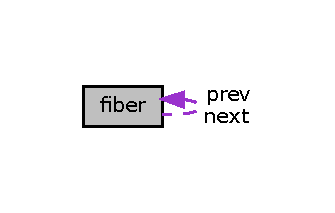
\includegraphics[width=161pt]{structfiber__coll__graph}
\end{center}
\end{figure}
\subsection*{Public Attributes}
\begin{DoxyCompactItemize}
\item 
\mbox{\hyperlink{core_8h_adb14c8b48a1d56cf9c6632295ab90048}{fiber\+\_\+node\+\_\+t}} $\ast$ \mbox{\hyperlink{structfiber_a327a77d565b2e0054f97b057e55b2178}{prev}}
\item 
\mbox{\hyperlink{core_8h_adb14c8b48a1d56cf9c6632295ab90048}{fiber\+\_\+node\+\_\+t}} $\ast$ \mbox{\hyperlink{structfiber_a8edc01f505460ec3df1f5319d26ee0cd}{next}}
\item 
unsigned \mbox{\hyperlink{structfiber_a6301190065f177d47b2d74fa1d1240c0}{id}}
\item 
\mbox{\Hypertarget{structfiber_a614a5ee08f9f0afe7f0b14b7fdb22437}\label{structfiber_a614a5ee08f9f0afe7f0b14b7fdb22437}} 
void $\ast$ {\bfseries starting\+\_\+function}
\item 
\mbox{\Hypertarget{structfiber_a3cf689305251f7117a3a91805f8ad729}\label{structfiber_a3cf689305251f7117a3a91805f8ad729}} 
unsigned long {\bfseries base\+\_\+user\+\_\+stack\+\_\+pointer}
\item 
\mbox{\Hypertarget{structfiber_a4ea650b723a810af6832f697a0de7e99}\label{structfiber_a4ea650b723a810af6832f697a0de7e99}} 
\mbox{\hyperlink{core_8h_a707fd6f68415e6978adb340746527715}{fiber\+\_\+state\+\_\+t}} {\bfseries state}
\item 
\mbox{\Hypertarget{structfiber_ae29b11c431ae8c5aa8e0c1e9027b28f2}\label{structfiber_ae29b11c431ae8c5aa8e0c1e9027b28f2}} 
struct pt\+\_\+regs {\bfseries regs}
\item 
\mbox{\Hypertarget{structfiber_adc6e3e51fa77df35cc927f1c088cee4e}\label{structfiber_adc6e3e51fa77df35cc927f1c088cee4e}} 
pid\+\_\+t {\bfseries created\+\_\+by}
\item 
\mbox{\Hypertarget{structfiber_a1e8bfeeac1b424ed9934df75aa294141}\label{structfiber_a1e8bfeeac1b424ed9934df75aa294141}} 
unsigned {\bfseries success\+\_\+activations\+\_\+count}
\item 
\mbox{\Hypertarget{structfiber_ac47ac73fa0666a3c6b2f7abe4963bc32}\label{structfiber_ac47ac73fa0666a3c6b2f7abe4963bc32}} 
unsigned {\bfseries failed\+\_\+activations\+\_\+count}
\item 
\mbox{\Hypertarget{structfiber_ac20c19c4679f14d5abad539853c42bc3}\label{structfiber_ac20c19c4679f14d5abad539853c42bc3}} 
unsigned long {\bfseries total\+\_\+time}
\end{DoxyCompactItemize}


\subsection{Detailed Description}
A node in the \mbox{\hyperlink{structfibers__list}{fibers\+\_\+list}}. This type fully represent a {\ttfamily fiber}. 

This is the complete description of a fiber. 

\subsection{Member Data Documentation}
\mbox{\Hypertarget{structfiber_a6301190065f177d47b2d74fa1d1240c0}\label{structfiber_a6301190065f177d47b2d74fa1d1240c0}} 
\index{fiber@{fiber}!id@{id}}
\index{id@{id}!fiber@{fiber}}
\subsubsection{\texorpdfstring{id}{id}}
{\footnotesize\ttfamily unsigned fiber\+::id}

Unique if of the fiber, used for \mbox{\Hypertarget{structfiber_a8edc01f505460ec3df1f5319d26ee0cd}\label{structfiber_a8edc01f505460ec3df1f5319d26ee0cd}} 
\index{fiber@{fiber}!next@{next}}
\index{next@{next}!fiber@{fiber}}
\subsubsection{\texorpdfstring{next}{next}}
{\footnotesize\ttfamily \mbox{\hyperlink{core_8h_adb14c8b48a1d56cf9c6632295ab90048}{fiber\+\_\+node\+\_\+t}}$\ast$ fiber\+::next}

Pointer to the next element in the list \mbox{\Hypertarget{structfiber_a327a77d565b2e0054f97b057e55b2178}\label{structfiber_a327a77d565b2e0054f97b057e55b2178}} 
\index{fiber@{fiber}!prev@{prev}}
\index{prev@{prev}!fiber@{fiber}}
\subsubsection{\texorpdfstring{prev}{prev}}
{\footnotesize\ttfamily \mbox{\hyperlink{core_8h_adb14c8b48a1d56cf9c6632295ab90048}{fiber\+\_\+node\+\_\+t}}$\ast$ fiber\+::prev}

Pointer to the previous element in the list 

The documentation for this struct was generated from the following file\+:\begin{DoxyCompactItemize}
\item 
include/\mbox{\hyperlink{core_8h}{core.\+h}}\end{DoxyCompactItemize}

\hypertarget{structfiber__dev}{}\section{fiber\+\_\+dev Struct Reference}
\label{structfiber__dev}\index{fiber\+\_\+dev@{fiber\+\_\+dev}}


The main structure of the fiber char device.  




{\ttfamily \#include $<$device.\+h$>$}

\subsection*{Public Attributes}
\begin{DoxyCompactItemize}
\item 
\mbox{\Hypertarget{structfiber__dev_ab886dc5f56901d33b28f4dc75478aa27}\label{structfiber__dev_ab886dc5f56901d33b28f4dc75478aa27}} 
struct miscdevice {\bfseries device}
\end{DoxyCompactItemize}


\subsection{Detailed Description}
The main structure of the fiber char device. 

The documentation for this struct was generated from the following file\+:\begin{DoxyCompactItemize}
\item 
include/\mbox{\hyperlink{device_8h}{device.\+h}}\end{DoxyCompactItemize}

\hypertarget{structfibered__process}{}\section{fibered\+\_\+process Struct Reference}
\label{structfibered__process}\index{fibered\+\_\+process@{fibered\+\_\+process}}


A node of the list of processes in \mbox{\hyperlink{structfibered__processes__list}{fibered\+\_\+processes\+\_\+list}}, a {\bfseries fiber-\/enabled} process.  




{\ttfamily \#include $<$core.\+h$>$}



Collaboration diagram for fibered\+\_\+process\+:
\nopagebreak
\begin{figure}[H]
\begin{center}
\leavevmode
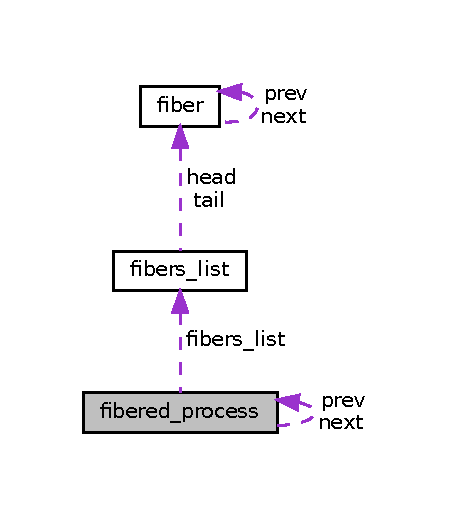
\includegraphics[width=216pt]{structfibered__process__coll__graph}
\end{center}
\end{figure}
\subsection*{Public Attributes}
\begin{DoxyCompactItemize}
\item 
\mbox{\hyperlink{core_8h_aa16708c717e33e5e95614cd1e4ca7b2b}{fibered\+\_\+process\+\_\+node\+\_\+t}} $\ast$ \mbox{\hyperlink{structfibered__process_adf5ba8614f416e75bc026fe449fdd08c}{prev}}
\item 
\mbox{\hyperlink{core_8h_aa16708c717e33e5e95614cd1e4ca7b2b}{fibered\+\_\+process\+\_\+node\+\_\+t}} $\ast$ \mbox{\hyperlink{structfibered__process_a8779fb1384900987ccd2d0d9de09a1ab}{next}}
\item 
\mbox{\hyperlink{core_8h_aad42420053a7ace7b3fb17805d6e9004}{fibers\+\_\+list\+\_\+t}} $\ast$ \mbox{\hyperlink{structfibered__process_a1aae0be425bbc05b6444909f16ec56b9}{fibers\+\_\+list}}
\item 
pid\+\_\+t \mbox{\hyperlink{structfibered__process_ad8f9adb6ee521988f3607ccf279e10a6}{pid}}
\end{DoxyCompactItemize}


\subsection{Detailed Description}
A node of the list of processes in \mbox{\hyperlink{structfibered__processes__list}{fibered\+\_\+processes\+\_\+list}}, a {\bfseries fiber-\/enabled} process. 

A \mbox{\hyperlink{structfibered__process}{fibered\+\_\+process}} is a process in which at least one thread has been converted to a fiber, so a \mbox{\hyperlink{structfibered__process}{fibered\+\_\+process}} always has at least one fiber in the \mbox{\hyperlink{structfibered__process_a1aae0be425bbc05b6444909f16ec56b9}{fibered\+\_\+process\+::fibers\+\_\+list}} field. Moreover the first element of the list has \mbox{\hyperlink{structfibered__process_adf5ba8614f416e75bc026fe449fdd08c}{fibered\+\_\+process\+::prev}} pointing to {\ttfamily N\+U\+LL} and the last element of the list has \mbox{\hyperlink{structfibered__process_a8779fb1384900987ccd2d0d9de09a1ab}{fibered\+\_\+process\+::next}} pointing to {\ttfamily N\+U\+LL}. 

\subsection{Member Data Documentation}
\mbox{\Hypertarget{structfibered__process_a1aae0be425bbc05b6444909f16ec56b9}\label{structfibered__process_a1aae0be425bbc05b6444909f16ec56b9}} 
\index{fibered\+\_\+process@{fibered\+\_\+process}!fibers\+\_\+list@{fibers\+\_\+list}}
\index{fibers\+\_\+list@{fibers\+\_\+list}!fibered\+\_\+process@{fibered\+\_\+process}}
\subsubsection{\texorpdfstring{fibers\+\_\+list}{fibers\_list}}
{\footnotesize\ttfamily \mbox{\hyperlink{core_8h_aad42420053a7ace7b3fb17805d6e9004}{fibers\+\_\+list\+\_\+t}}$\ast$ fibered\+\_\+process\+::fibers\+\_\+list}

A list of fibers created in the process environment (so by any thread in it) \mbox{\Hypertarget{structfibered__process_a8779fb1384900987ccd2d0d9de09a1ab}\label{structfibered__process_a8779fb1384900987ccd2d0d9de09a1ab}} 
\index{fibered\+\_\+process@{fibered\+\_\+process}!next@{next}}
\index{next@{next}!fibered\+\_\+process@{fibered\+\_\+process}}
\subsubsection{\texorpdfstring{next}{next}}
{\footnotesize\ttfamily \mbox{\hyperlink{core_8h_aa16708c717e33e5e95614cd1e4ca7b2b}{fibered\+\_\+process\+\_\+node\+\_\+t}}$\ast$ fibered\+\_\+process\+::next}

The next element of the list \mbox{\Hypertarget{structfibered__process_ad8f9adb6ee521988f3607ccf279e10a6}\label{structfibered__process_ad8f9adb6ee521988f3607ccf279e10a6}} 
\index{fibered\+\_\+process@{fibered\+\_\+process}!pid@{pid}}
\index{pid@{pid}!fibered\+\_\+process@{fibered\+\_\+process}}
\subsubsection{\texorpdfstring{pid}{pid}}
{\footnotesize\ttfamily pid\+\_\+t fibered\+\_\+process\+::pid}

the pid of the main thread, so the tgid of every thread of the process \mbox{\Hypertarget{structfibered__process_adf5ba8614f416e75bc026fe449fdd08c}\label{structfibered__process_adf5ba8614f416e75bc026fe449fdd08c}} 
\index{fibered\+\_\+process@{fibered\+\_\+process}!prev@{prev}}
\index{prev@{prev}!fibered\+\_\+process@{fibered\+\_\+process}}
\subsubsection{\texorpdfstring{prev}{prev}}
{\footnotesize\ttfamily \mbox{\hyperlink{core_8h_aa16708c717e33e5e95614cd1e4ca7b2b}{fibered\+\_\+process\+\_\+node\+\_\+t}}$\ast$ fibered\+\_\+process\+::prev}

The previous element of the list 

The documentation for this struct was generated from the following file\+:\begin{DoxyCompactItemize}
\item 
include/\mbox{\hyperlink{core_8h}{core.\+h}}\end{DoxyCompactItemize}

\hypertarget{structfibered__processes__list}{}\section{fibered\+\_\+processes\+\_\+list Struct Reference}
\label{structfibered__processes__list}\index{fibered\+\_\+processes\+\_\+list@{fibered\+\_\+processes\+\_\+list}}


The list of processes that have at least one fiber.  




{\ttfamily \#include $<$core.\+h$>$}



Collaboration diagram for fibered\+\_\+processes\+\_\+list\+:
\nopagebreak
\begin{figure}[H]
\begin{center}
\leavevmode
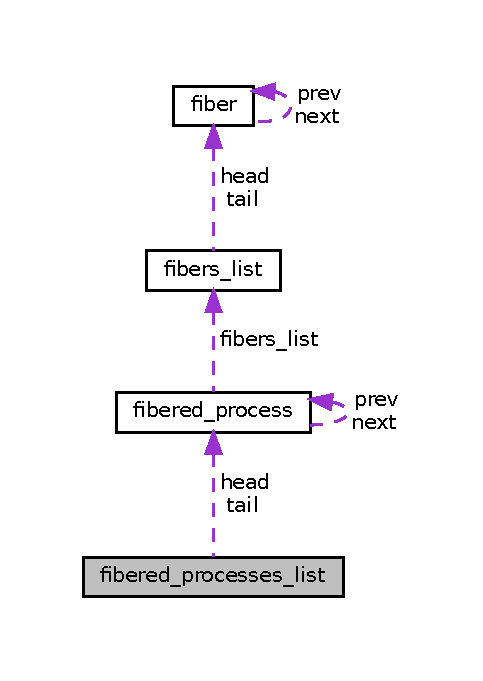
\includegraphics[width=232pt]{structfibered__processes__list__coll__graph}
\end{center}
\end{figure}
\subsection*{Public Attributes}
\begin{DoxyCompactItemize}
\item 
\mbox{\hyperlink{core_8h_aa16708c717e33e5e95614cd1e4ca7b2b}{fibered\+\_\+process\+\_\+node\+\_\+t}} $\ast$ \mbox{\hyperlink{structfibered__processes__list_a460c3f34099c7589c25c383add98650b}{head}}
\item 
\mbox{\hyperlink{core_8h_aa16708c717e33e5e95614cd1e4ca7b2b}{fibered\+\_\+process\+\_\+node\+\_\+t}} $\ast$ \mbox{\hyperlink{structfibered__processes__list_a423b95d461fa440ede7dd019b8c94aa6}{tail}}
\item 
unsigned \mbox{\hyperlink{structfibered__processes__list_a357ed70a414391e2cde4cf1c6062b6ce}{processes\+\_\+count}}
\end{DoxyCompactItemize}


\subsection{Detailed Description}
The list of processes that have at least one fiber. 

This list has the purpose of containing the list of processes that have created at least one fiber and they became fiber-\/enabled. The list can be considered empty when at least one of \mbox{\hyperlink{structfibered__processes__list_a460c3f34099c7589c25c383add98650b}{fibered\+\_\+processes\+\_\+list\+::head}} or \mbox{\hyperlink{structfibered__processes__list_a423b95d461fa440ede7dd019b8c94aa6}{fibered\+\_\+processes\+\_\+list\+::tail}} is pointing to {\ttfamily N\+U\+LL}. 

\subsection{Member Data Documentation}
\mbox{\Hypertarget{structfibered__processes__list_a460c3f34099c7589c25c383add98650b}\label{structfibered__processes__list_a460c3f34099c7589c25c383add98650b}} 
\index{fibered\+\_\+processes\+\_\+list@{fibered\+\_\+processes\+\_\+list}!head@{head}}
\index{head@{head}!fibered\+\_\+processes\+\_\+list@{fibered\+\_\+processes\+\_\+list}}
\subsubsection{\texorpdfstring{head}{head}}
{\footnotesize\ttfamily \mbox{\hyperlink{core_8h_aa16708c717e33e5e95614cd1e4ca7b2b}{fibered\+\_\+process\+\_\+node\+\_\+t}}$\ast$ fibered\+\_\+processes\+\_\+list\+::head}

The first element in the list \mbox{\Hypertarget{structfibered__processes__list_a357ed70a414391e2cde4cf1c6062b6ce}\label{structfibered__processes__list_a357ed70a414391e2cde4cf1c6062b6ce}} 
\index{fibered\+\_\+processes\+\_\+list@{fibered\+\_\+processes\+\_\+list}!processes\+\_\+count@{processes\+\_\+count}}
\index{processes\+\_\+count@{processes\+\_\+count}!fibered\+\_\+processes\+\_\+list@{fibered\+\_\+processes\+\_\+list}}
\subsubsection{\texorpdfstring{processes\+\_\+count}{processes\_count}}
{\footnotesize\ttfamily unsigned fibered\+\_\+processes\+\_\+list\+::processes\+\_\+count}

The number of elements in the list \mbox{\Hypertarget{structfibered__processes__list_a423b95d461fa440ede7dd019b8c94aa6}\label{structfibered__processes__list_a423b95d461fa440ede7dd019b8c94aa6}} 
\index{fibered\+\_\+processes\+\_\+list@{fibered\+\_\+processes\+\_\+list}!tail@{tail}}
\index{tail@{tail}!fibered\+\_\+processes\+\_\+list@{fibered\+\_\+processes\+\_\+list}}
\subsubsection{\texorpdfstring{tail}{tail}}
{\footnotesize\ttfamily \mbox{\hyperlink{core_8h_aa16708c717e33e5e95614cd1e4ca7b2b}{fibered\+\_\+process\+\_\+node\+\_\+t}}$\ast$ fibered\+\_\+processes\+\_\+list\+::tail}

The last element in the list 

The documentation for this struct was generated from the following file\+:\begin{DoxyCompactItemize}
\item 
include/\mbox{\hyperlink{core_8h}{core.\+h}}\end{DoxyCompactItemize}

\hypertarget{structfibers__list}{}\section{fibers\+\_\+list Struct Reference}
\label{structfibers__list}\index{fibers\+\_\+list@{fibers\+\_\+list}}


A generic list of fibers.  




{\ttfamily \#include $<$core.\+h$>$}



Collaboration diagram for fibers\+\_\+list\+:
\nopagebreak
\begin{figure}[H]
\begin{center}
\leavevmode
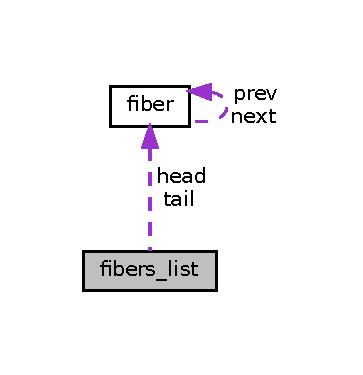
\includegraphics[width=174pt]{structfibers__list__coll__graph}
\end{center}
\end{figure}
\subsection*{Public Attributes}
\begin{DoxyCompactItemize}
\item 
\mbox{\hyperlink{core_8h_adb14c8b48a1d56cf9c6632295ab90048}{fiber\+\_\+node\+\_\+t}} $\ast$ \mbox{\hyperlink{structfibers__list_aa1dd39c8c192607d164f204821d5b3ed}{head}}
\item 
\mbox{\hyperlink{core_8h_adb14c8b48a1d56cf9c6632295ab90048}{fiber\+\_\+node\+\_\+t}} $\ast$ \mbox{\hyperlink{structfibers__list_af94c6bcedeb27c078ea1fa4869c53673}{tail}}
\item 
unsigned \mbox{\hyperlink{structfibers__list_a54a8a9f5a97c783b1461257d6e07aa1a}{fibers\+\_\+count}}
\end{DoxyCompactItemize}


\subsection{Detailed Description}
A generic list of fibers. 

The list has the purpose of containing the list of fibers for a given process. The list can be considered empty when at least one of \mbox{\hyperlink{structfibers__list_aa1dd39c8c192607d164f204821d5b3ed}{fibers\+\_\+list\+::head}} or \mbox{\hyperlink{structfibers__list_af94c6bcedeb27c078ea1fa4869c53673}{fibers\+\_\+list\+::tail}} is pointing to {\ttfamily N\+U\+LL}. 

\subsection{Member Data Documentation}
\mbox{\Hypertarget{structfibers__list_a54a8a9f5a97c783b1461257d6e07aa1a}\label{structfibers__list_a54a8a9f5a97c783b1461257d6e07aa1a}} 
\index{fibers\+\_\+list@{fibers\+\_\+list}!fibers\+\_\+count@{fibers\+\_\+count}}
\index{fibers\+\_\+count@{fibers\+\_\+count}!fibers\+\_\+list@{fibers\+\_\+list}}
\subsubsection{\texorpdfstring{fibers\+\_\+count}{fibers\_count}}
{\footnotesize\ttfamily unsigned fibers\+\_\+list\+::fibers\+\_\+count}

Number of fibers created \mbox{\Hypertarget{structfibers__list_aa1dd39c8c192607d164f204821d5b3ed}\label{structfibers__list_aa1dd39c8c192607d164f204821d5b3ed}} 
\index{fibers\+\_\+list@{fibers\+\_\+list}!head@{head}}
\index{head@{head}!fibers\+\_\+list@{fibers\+\_\+list}}
\subsubsection{\texorpdfstring{head}{head}}
{\footnotesize\ttfamily \mbox{\hyperlink{core_8h_adb14c8b48a1d56cf9c6632295ab90048}{fiber\+\_\+node\+\_\+t}}$\ast$ fibers\+\_\+list\+::head}

The first element in the list \mbox{\Hypertarget{structfibers__list_af94c6bcedeb27c078ea1fa4869c53673}\label{structfibers__list_af94c6bcedeb27c078ea1fa4869c53673}} 
\index{fibers\+\_\+list@{fibers\+\_\+list}!tail@{tail}}
\index{tail@{tail}!fibers\+\_\+list@{fibers\+\_\+list}}
\subsubsection{\texorpdfstring{tail}{tail}}
{\footnotesize\ttfamily \mbox{\hyperlink{core_8h_adb14c8b48a1d56cf9c6632295ab90048}{fiber\+\_\+node\+\_\+t}}$\ast$ fibers\+\_\+list\+::tail}

The last element in the list 

The documentation for this struct was generated from the following file\+:\begin{DoxyCompactItemize}
\item 
include/\mbox{\hyperlink{core_8h}{core.\+h}}\end{DoxyCompactItemize}

\chapter{File Documentation}
\hypertarget{core_8h}{}\section{include/core.h File Reference}
\label{core_8h}\index{include/core.\+h@{include/core.\+h}}


The head of the core part of the module.  


{\ttfamily \#include \char`\"{}common.\+h\char`\"{}}\newline
{\ttfamily \#include \char`\"{}ioctlcmd.\+h\char`\"{}}\newline
{\ttfamily \#include $<$asm/current.\+h$>$}\newline
{\ttfamily \#include $<$asm/ptrace.\+h$>$}\newline
{\ttfamily \#include $<$linux/fs.\+h$>$}\newline
{\ttfamily \#include $<$linux/hashtable.\+h$>$}\newline
{\ttfamily \#include $<$linux/ioctl.\+h$>$}\newline
{\ttfamily \#include $<$linux/kernel.\+h$>$}\newline
{\ttfamily \#include $<$linux/list.\+h$>$}\newline
{\ttfamily \#include $<$linux/module.\+h$>$}\newline
{\ttfamily \#include $<$linux/sched/task\+\_\+stack.\+h$>$}\newline
{\ttfamily \#include $<$linux/semaphore.\+h$>$}\newline
{\ttfamily \#include $<$linux/slab.\+h$>$}\newline
{\ttfamily \#include $<$linux/uaccess.\+h$>$}\newline
Include dependency graph for core.\+h\+:
\nopagebreak
\begin{figure}[H]
\begin{center}
\leavevmode
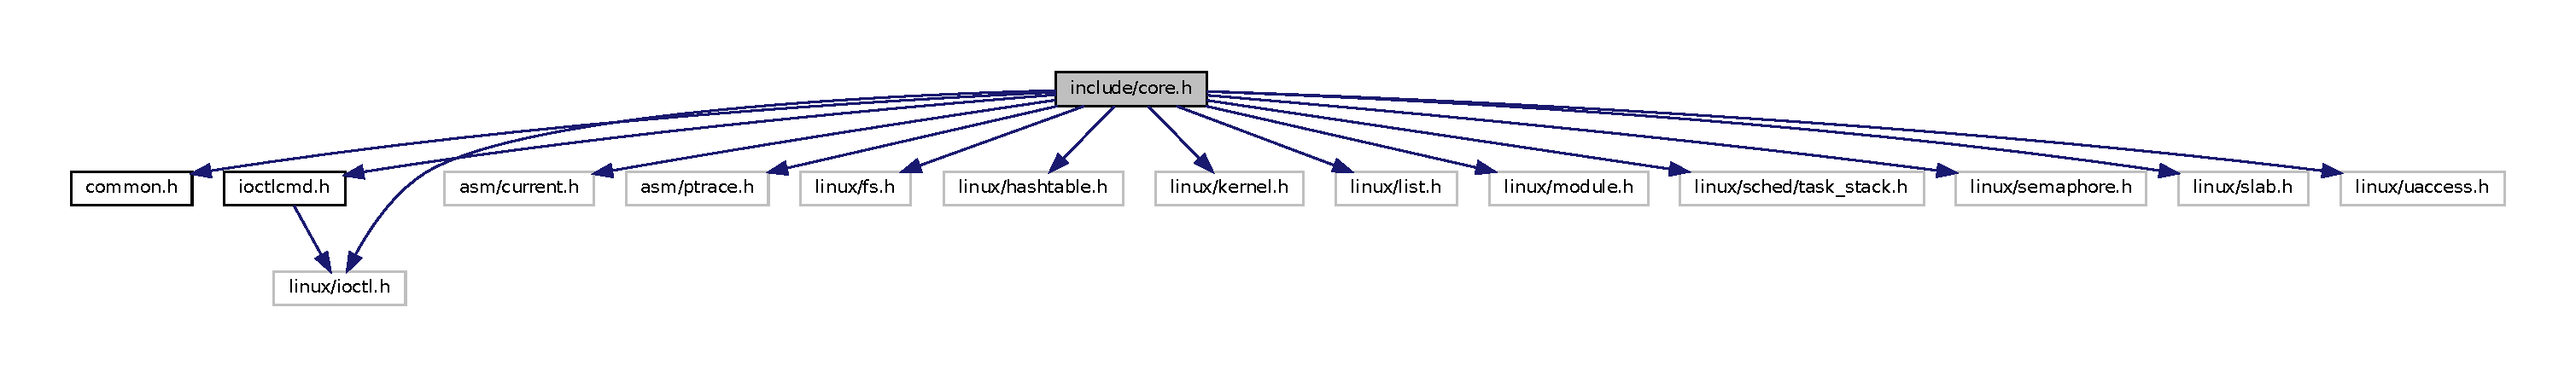
\includegraphics[width=350pt]{core_8h__incl}
\end{center}
\end{figure}
This graph shows which files directly or indirectly include this file\+:
\nopagebreak
\begin{figure}[H]
\begin{center}
\leavevmode
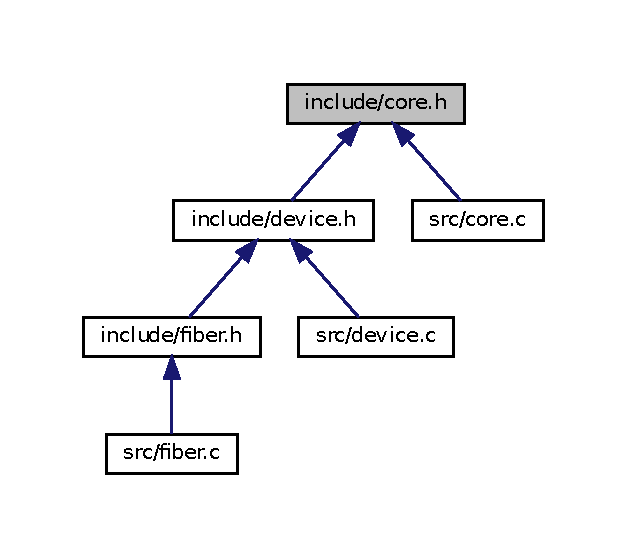
\includegraphics[width=301pt]{core_8h__dep__incl}
\end{center}
\end{figure}
\subsection*{Classes}
\begin{DoxyCompactItemize}
\item 
struct \mbox{\hyperlink{structfibered__process}{fibered\+\_\+process}}
\begin{DoxyCompactList}\small\item\em A node of the list of processes in \mbox{\hyperlink{structfibered__processes__list}{fibered\+\_\+processes\+\_\+list}}, a {\bfseries fiber-\/enabled} process. \end{DoxyCompactList}\item 
struct \mbox{\hyperlink{structfibered__processes__list}{fibered\+\_\+processes\+\_\+list}}
\begin{DoxyCompactList}\small\item\em The list of processes that have at least one fiber. \end{DoxyCompactList}\item 
struct \mbox{\hyperlink{structfiber}{fiber}}
\begin{DoxyCompactList}\small\item\em A node in the \mbox{\hyperlink{structfibers__list}{fibers\+\_\+list}}. This type fully represent a {\ttfamily fiber}. \end{DoxyCompactList}\item 
struct \mbox{\hyperlink{structfibers__list}{fibers\+\_\+list}}
\begin{DoxyCompactList}\small\item\em A generic list of fibers. \end{DoxyCompactList}\end{DoxyCompactItemize}
\subsection*{Macros}
\begin{DoxyCompactItemize}
\item 
\mbox{\Hypertarget{core_8h_a88633244fc905d1234bac90e464791da}\label{core_8h_a88633244fc905d1234bac90e464791da}} 
\#define {\bfseries E\+R\+R\+\_\+\+T\+H\+R\+E\+A\+D\+\_\+\+A\+L\+R\+E\+A\+D\+Y\+\_\+\+F\+I\+B\+ER}~100
\item 
\mbox{\Hypertarget{core_8h_a4cc9121f26b7a012965835e97dfd5315}\label{core_8h_a4cc9121f26b7a012965835e97dfd5315}} 
\#define {\bfseries C\+O\+R\+E\+\_\+\+L\+OG}~\char`\"{}\+: D\+E\+V\+: \char`\"{}
\end{DoxyCompactItemize}
\subsection*{Typedefs}
\begin{DoxyCompactItemize}
\item 
typedef struct \mbox{\hyperlink{structfibered__process}{fibered\+\_\+process}} \mbox{\hyperlink{core_8h_aa16708c717e33e5e95614cd1e4ca7b2b}{fibered\+\_\+process\+\_\+node\+\_\+t}}
\begin{DoxyCompactList}\small\item\em A node of the list of processes in \mbox{\hyperlink{structfibered__processes__list}{fibered\+\_\+processes\+\_\+list}}, a {\bfseries fiber-\/enabled} process. \end{DoxyCompactList}\item 
\mbox{\Hypertarget{core_8h_a87e2a324967b7142f288286f66f2a149}\label{core_8h_a87e2a324967b7142f288286f66f2a149}} 
typedef struct fiber\+\_\+processes\+\_\+list {\bfseries fiber\+\_\+process\+\_\+list\+\_\+t}
\item 
typedef struct \mbox{\hyperlink{structfiber}{fiber}} \mbox{\hyperlink{core_8h_adb14c8b48a1d56cf9c6632295ab90048}{fiber\+\_\+node\+\_\+t}}
\begin{DoxyCompactList}\small\item\em A node in the \mbox{\hyperlink{structfibers__list}{fibers\+\_\+list}}. This type fully represent a {\ttfamily fiber}. \end{DoxyCompactList}\item 
typedef struct \mbox{\hyperlink{structfibers__list}{fibers\+\_\+list}} \mbox{\hyperlink{core_8h_aad42420053a7ace7b3fb17805d6e9004}{fibers\+\_\+list\+\_\+t}}
\begin{DoxyCompactList}\small\item\em A generic list of fibers. \end{DoxyCompactList}\item 
\mbox{\Hypertarget{core_8h_a707fd6f68415e6978adb340746527715}\label{core_8h_a707fd6f68415e6978adb340746527715}} 
typedef enum \mbox{\hyperlink{core_8h_a7b11bd960a2de8da146a5ebb7f7abbc2}{fiber\+\_\+state}} \mbox{\hyperlink{core_8h_a707fd6f68415e6978adb340746527715}{fiber\+\_\+state\+\_\+t}}
\begin{DoxyCompactList}\small\item\em The state of the fiber. \end{DoxyCompactList}\item 
typedef struct \mbox{\hyperlink{structfibered__processes__list}{fibered\+\_\+processes\+\_\+list}} \mbox{\hyperlink{core_8h_afffa2dfe134b8b5494026f1038f68a39}{fibered\+\_\+processes\+\_\+list\+\_\+t}}
\begin{DoxyCompactList}\small\item\em The list of processes that have at least one fiber. \end{DoxyCompactList}\end{DoxyCompactItemize}
\subsection*{Enumerations}
\begin{DoxyCompactItemize}
\item 
enum \mbox{\hyperlink{core_8h_a7b11bd960a2de8da146a5ebb7f7abbc2}{fiber\+\_\+state}} \{ \mbox{\hyperlink{core_8h_a7b11bd960a2de8da146a5ebb7f7abbc2a1061be6c3fb88d32829cba6f6b2be304}{R\+U\+N\+N\+I\+NG}}, 
\mbox{\hyperlink{core_8h_a7b11bd960a2de8da146a5ebb7f7abbc2afd6a0e4343048b10646dd2976cc5ad18}{I\+D\+LE}}
 \}
\begin{DoxyCompactList}\small\item\em The state of the fiber. \end{DoxyCompactList}\end{DoxyCompactItemize}
\subsection*{Functions}
\begin{DoxyCompactItemize}
\item 
int \mbox{\hyperlink{core_8h_a62235692d124309201f915bec1a89374}{convert\+\_\+thread\+\_\+to\+\_\+fiber}} (void)
\begin{DoxyCompactList}\small\item\em Convert the current thread to a fiber. \end{DoxyCompactList}\end{DoxyCompactItemize}


\subsection{Detailed Description}
The head of the core part of the module. 

This file contains all the data structures and the methods that implements the core functions of the fiber module

\begin{DoxyAuthor}{Author}
Gabriele Proietti Mattia \href{mailto:gabry.gabry@hotmail.it}{\tt gabry.\+gabry@hotmail.\+it} 

Alexandru Daniel Tufa \href{mailto:alex.tufa94@gmail.com}{\tt alex.\+tufa94@gmail.\+com} 
\end{DoxyAuthor}
\begin{DoxyDate}{Date}
2018-\/05-\/13 
\end{DoxyDate}


\subsection{Typedef Documentation}
\mbox{\Hypertarget{core_8h_adb14c8b48a1d56cf9c6632295ab90048}\label{core_8h_adb14c8b48a1d56cf9c6632295ab90048}} 
\index{core.\+h@{core.\+h}!fiber\+\_\+node\+\_\+t@{fiber\+\_\+node\+\_\+t}}
\index{fiber\+\_\+node\+\_\+t@{fiber\+\_\+node\+\_\+t}!core.\+h@{core.\+h}}
\subsubsection{\texorpdfstring{fiber\+\_\+node\+\_\+t}{fiber\_node\_t}}
{\footnotesize\ttfamily typedef struct \mbox{\hyperlink{structfiber}{fiber}} \mbox{\hyperlink{core_8h_adb14c8b48a1d56cf9c6632295ab90048}{fiber\+\_\+node\+\_\+t}}}



A node in the \mbox{\hyperlink{structfibers__list}{fibers\+\_\+list}}. This type fully represent a {\ttfamily fiber}. 

This is the complete description of a fiber. \mbox{\Hypertarget{core_8h_aa16708c717e33e5e95614cd1e4ca7b2b}\label{core_8h_aa16708c717e33e5e95614cd1e4ca7b2b}} 
\index{core.\+h@{core.\+h}!fibered\+\_\+process\+\_\+node\+\_\+t@{fibered\+\_\+process\+\_\+node\+\_\+t}}
\index{fibered\+\_\+process\+\_\+node\+\_\+t@{fibered\+\_\+process\+\_\+node\+\_\+t}!core.\+h@{core.\+h}}
\subsubsection{\texorpdfstring{fibered\+\_\+process\+\_\+node\+\_\+t}{fibered\_process\_node\_t}}
{\footnotesize\ttfamily typedef struct \mbox{\hyperlink{structfibered__process}{fibered\+\_\+process}} \mbox{\hyperlink{core_8h_aa16708c717e33e5e95614cd1e4ca7b2b}{fibered\+\_\+process\+\_\+node\+\_\+t}}}



A node of the list of processes in \mbox{\hyperlink{structfibered__processes__list}{fibered\+\_\+processes\+\_\+list}}, a {\bfseries fiber-\/enabled} process. 

A \mbox{\hyperlink{structfibered__process}{fibered\+\_\+process}} is a process in which at least one thread has been converted to a fiber, so a \mbox{\hyperlink{structfibered__process}{fibered\+\_\+process}} always has at least one fiber in the \mbox{\hyperlink{structfibered__process_a1aae0be425bbc05b6444909f16ec56b9}{fibered\+\_\+process\+::fibers\+\_\+list}} field. Moreover the first element of the list has \mbox{\hyperlink{structfibered__process_adf5ba8614f416e75bc026fe449fdd08c}{fibered\+\_\+process\+::prev}} pointing to {\ttfamily N\+U\+LL} and the last element of the list has \mbox{\hyperlink{structfibered__process_a8779fb1384900987ccd2d0d9de09a1ab}{fibered\+\_\+process\+::next}} pointing to {\ttfamily N\+U\+LL}. \mbox{\Hypertarget{core_8h_afffa2dfe134b8b5494026f1038f68a39}\label{core_8h_afffa2dfe134b8b5494026f1038f68a39}} 
\index{core.\+h@{core.\+h}!fibered\+\_\+processes\+\_\+list\+\_\+t@{fibered\+\_\+processes\+\_\+list\+\_\+t}}
\index{fibered\+\_\+processes\+\_\+list\+\_\+t@{fibered\+\_\+processes\+\_\+list\+\_\+t}!core.\+h@{core.\+h}}
\subsubsection{\texorpdfstring{fibered\+\_\+processes\+\_\+list\+\_\+t}{fibered\_processes\_list\_t}}
{\footnotesize\ttfamily typedef struct \mbox{\hyperlink{structfibered__processes__list}{fibered\+\_\+processes\+\_\+list}}  \mbox{\hyperlink{core_8h_afffa2dfe134b8b5494026f1038f68a39}{fibered\+\_\+processes\+\_\+list\+\_\+t}}}



The list of processes that have at least one fiber. 

This list has the purpose of containing the list of processes that have created at least one fiber and they became fiber-\/enabled. The list can be considered empty when at least one of \mbox{\hyperlink{structfibered__processes__list_a460c3f34099c7589c25c383add98650b}{fibered\+\_\+processes\+\_\+list\+::head}} or \mbox{\hyperlink{structfibered__processes__list_a423b95d461fa440ede7dd019b8c94aa6}{fibered\+\_\+processes\+\_\+list\+::tail}} is pointing to {\ttfamily N\+U\+LL}. \mbox{\Hypertarget{core_8h_aad42420053a7ace7b3fb17805d6e9004}\label{core_8h_aad42420053a7ace7b3fb17805d6e9004}} 
\index{core.\+h@{core.\+h}!fibers\+\_\+list\+\_\+t@{fibers\+\_\+list\+\_\+t}}
\index{fibers\+\_\+list\+\_\+t@{fibers\+\_\+list\+\_\+t}!core.\+h@{core.\+h}}
\subsubsection{\texorpdfstring{fibers\+\_\+list\+\_\+t}{fibers\_list\_t}}
{\footnotesize\ttfamily typedef struct \mbox{\hyperlink{structfibers__list}{fibers\+\_\+list}} \mbox{\hyperlink{core_8h_aad42420053a7ace7b3fb17805d6e9004}{fibers\+\_\+list\+\_\+t}}}



A generic list of fibers. 

The list has the purpose of containing the list of fibers for a given process. The list can be considered empty when at least one of \mbox{\hyperlink{structfibers__list_aa1dd39c8c192607d164f204821d5b3ed}{fibers\+\_\+list\+::head}} or \mbox{\hyperlink{structfibers__list_af94c6bcedeb27c078ea1fa4869c53673}{fibers\+\_\+list\+::tail}} is pointing to {\ttfamily N\+U\+LL}. 

\subsection{Enumeration Type Documentation}
\mbox{\Hypertarget{core_8h_a7b11bd960a2de8da146a5ebb7f7abbc2}\label{core_8h_a7b11bd960a2de8da146a5ebb7f7abbc2}} 
\index{core.\+h@{core.\+h}!fiber\+\_\+state@{fiber\+\_\+state}}
\index{fiber\+\_\+state@{fiber\+\_\+state}!core.\+h@{core.\+h}}
\subsubsection{\texorpdfstring{fiber\+\_\+state}{fiber\_state}}
{\footnotesize\ttfamily enum \mbox{\hyperlink{core_8h_a7b11bd960a2de8da146a5ebb7f7abbc2}{fiber\+\_\+state}}}



The state of the fiber. 

\begin{DoxyEnumFields}{Enumerator}
\raisebox{\heightof{T}}[0pt][0pt]{\index{R\+U\+N\+N\+I\+NG@{R\+U\+N\+N\+I\+NG}!core.\+h@{core.\+h}}\index{core.\+h@{core.\+h}!R\+U\+N\+N\+I\+NG@{R\+U\+N\+N\+I\+NG}}}\mbox{\Hypertarget{core_8h_a7b11bd960a2de8da146a5ebb7f7abbc2a1061be6c3fb88d32829cba6f6b2be304}\label{core_8h_a7b11bd960a2de8da146a5ebb7f7abbc2a1061be6c3fb88d32829cba6f6b2be304}} 
R\+U\+N\+N\+I\+NG&The fiber is running since the thread switched to it \\
\hline

\raisebox{\heightof{T}}[0pt][0pt]{\index{I\+D\+LE@{I\+D\+LE}!core.\+h@{core.\+h}}\index{core.\+h@{core.\+h}!I\+D\+LE@{I\+D\+LE}}}\mbox{\Hypertarget{core_8h_a7b11bd960a2de8da146a5ebb7f7abbc2afd6a0e4343048b10646dd2976cc5ad18}\label{core_8h_a7b11bd960a2de8da146a5ebb7f7abbc2afd6a0e4343048b10646dd2976cc5ad18}} 
I\+D\+LE&The fiber is created but no thread switched to it \\
\hline

\end{DoxyEnumFields}


\subsection{Function Documentation}
\mbox{\Hypertarget{core_8h_a62235692d124309201f915bec1a89374}\label{core_8h_a62235692d124309201f915bec1a89374}} 
\index{core.\+h@{core.\+h}!convert\+\_\+thread\+\_\+to\+\_\+fiber@{convert\+\_\+thread\+\_\+to\+\_\+fiber}}
\index{convert\+\_\+thread\+\_\+to\+\_\+fiber@{convert\+\_\+thread\+\_\+to\+\_\+fiber}!core.\+h@{core.\+h}}
\subsubsection{\texorpdfstring{convert\+\_\+thread\+\_\+to\+\_\+fiber()}{convert\_thread\_to\_fiber()}}
{\footnotesize\ttfamily int convert\+\_\+thread\+\_\+to\+\_\+fiber (\begin{DoxyParamCaption}\item[{void}]{ }\end{DoxyParamCaption})}



Convert the current thread to a fiber. 

\subsection*{Implementation}

When a thread is converted to a fiber several task are performed. First of all, if the process never created a fiber, it must become {\bfseries fiber-\/enabled}, this means that we have to instantiate a \mbox{\hyperlink{structfibered__process}{fibered\+\_\+process}} element in the \mbox{\hyperlink{structfibered__processes__list}{fibered\+\_\+processes\+\_\+list}} variable. Then we have to instantiate a \mbox{\hyperlink{structfiber}{fiber}} element in the \mbox{\hyperlink{structfibers__list}{fibers\+\_\+list}} field of the \mbox{\hyperlink{structfibered__process}{fibered\+\_\+process}} element of the list.

\begin{DoxyReturn}{Returns}
int 0 if everything ok, otherwise an error listed in \mbox{\hyperlink{ioctlcmd_8h}{ioctlcmd.\+h}} 
\end{DoxyReturn}

\hypertarget{device_8h}{}\section{include/device.h File Reference}
\label{device_8h}\index{include/device.\+h@{include/device.\+h}}


This file contains definitions and macros for the {\itshape device} of the module.  


{\ttfamily \#include \char`\"{}common.\+h\char`\"{}}\newline
{\ttfamily \#include \char`\"{}core.\+h\char`\"{}}\newline
{\ttfamily \#include \char`\"{}ioctlcmd.\+h\char`\"{}}\newline
{\ttfamily \#include $<$asm/current.\+h$>$}\newline
{\ttfamily \#include $<$asm/ptrace.\+h$>$}\newline
{\ttfamily \#include $<$linux/cdev.\+h$>$}\newline
{\ttfamily \#include $<$linux/fs.\+h$>$}\newline
{\ttfamily \#include $<$linux/hashtable.\+h$>$}\newline
{\ttfamily \#include $<$linux/ioctl.\+h$>$}\newline
{\ttfamily \#include $<$linux/kernel.\+h$>$}\newline
{\ttfamily \#include $<$linux/miscdevice.\+h$>$}\newline
{\ttfamily \#include $<$linux/module.\+h$>$}\newline
{\ttfamily \#include $<$linux/sched/task\+\_\+stack.\+h$>$}\newline
{\ttfamily \#include $<$linux/semaphore.\+h$>$}\newline
{\ttfamily \#include $<$linux/slab.\+h$>$}\newline
{\ttfamily \#include $<$linux/uaccess.\+h$>$}\newline
Include dependency graph for device.\+h\+:
\nopagebreak
\begin{figure}[H]
\begin{center}
\leavevmode
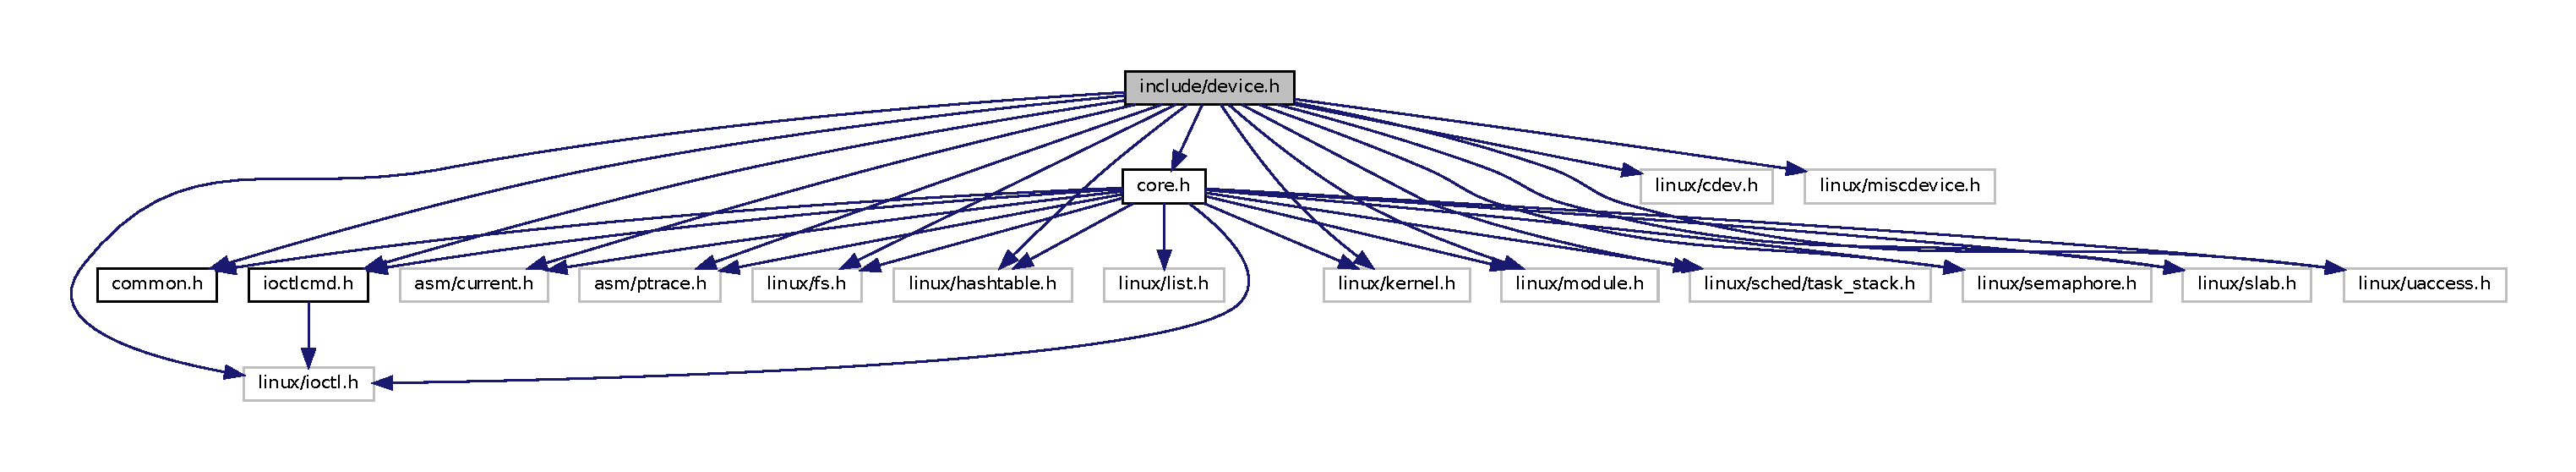
\includegraphics[width=350pt]{device_8h__incl}
\end{center}
\end{figure}
This graph shows which files directly or indirectly include this file\+:
\nopagebreak
\begin{figure}[H]
\begin{center}
\leavevmode
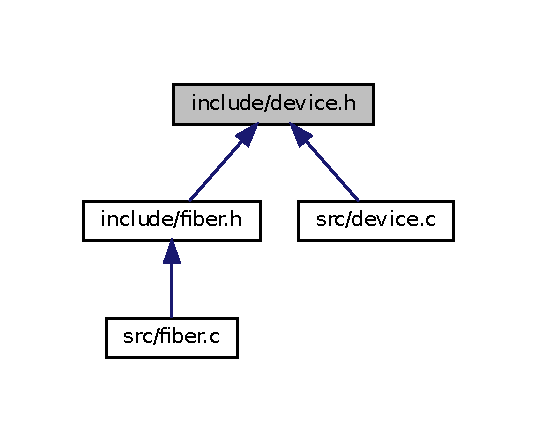
\includegraphics[width=258pt]{device_8h__dep__incl}
\end{center}
\end{figure}
\subsection*{Classes}
\begin{DoxyCompactItemize}
\item 
struct \mbox{\hyperlink{structfiber__dev}{fiber\+\_\+dev}}
\begin{DoxyCompactList}\small\item\em The main structure of the fiber char device. \end{DoxyCompactList}\end{DoxyCompactItemize}
\subsection*{Macros}
\begin{DoxyCompactItemize}
\item 
\mbox{\Hypertarget{device_8h_a64f0bd23927c33ab55469a5f2e17bff6}\label{device_8h_a64f0bd23927c33ab55469a5f2e17bff6}} 
\#define {\bfseries D\+E\+V\+I\+C\+E\+\_\+\+L\+OG}~\char`\"{}\+: D\+E\+V\+: \char`\"{}
\item 
\mbox{\Hypertarget{device_8h_a062eed9032d965350a8de227131182e7}\label{device_8h_a062eed9032d965350a8de227131182e7}} 
\#define {\bfseries F\+I\+B\+E\+R\+\_\+\+D\+E\+V\+I\+C\+E\+\_\+\+N\+A\+ME}~\char`\"{}fiber\char`\"{}
\item 
\mbox{\Hypertarget{device_8h_a8b5839f71a3b6e7d64b2d5e9967e3dd1}\label{device_8h_a8b5839f71a3b6e7d64b2d5e9967e3dd1}} 
\#define {\bfseries B\+U\+F\+\_\+\+L\+EN}~80
\end{DoxyCompactItemize}
\subsection*{Typedefs}
\begin{DoxyCompactItemize}
\item 
\mbox{\Hypertarget{device_8h_ad8cf304de032bd5afa605f8bbbc8ff63}\label{device_8h_ad8cf304de032bd5afa605f8bbbc8ff63}} 
typedef struct \mbox{\hyperlink{structfiber__dev}{fiber\+\_\+dev}} \mbox{\hyperlink{device_8h_ad8cf304de032bd5afa605f8bbbc8ff63}{fiber\+\_\+dev\+\_\+t}}
\begin{DoxyCompactList}\small\item\em The main structure of the fiber char device. \end{DoxyCompactList}\end{DoxyCompactItemize}
\subsection*{Functions}
\begin{DoxyCompactItemize}
\item 
int \mbox{\hyperlink{device_8h_a88bd4adb20dc9040ae78f5b4036b61ab}{init\+\_\+device}} (void)
\begin{DoxyCompactList}\small\item\em Init the device inspired by \href{https://www.linuxjournal.com/article/2920}{\tt https\+://www.\+linuxjournal.\+com/article/2920}. \end{DoxyCompactList}\item 
\mbox{\Hypertarget{device_8h_a80ad9d4cfc87c34e428952a2d24b73e5}\label{device_8h_a80ad9d4cfc87c34e428952a2d24b73e5}} 
void \mbox{\hyperlink{device_8h_a80ad9d4cfc87c34e428952a2d24b73e5}{destroy\+\_\+device}} (void)
\begin{DoxyCompactList}\small\item\em Destroy the device. \end{DoxyCompactList}\end{DoxyCompactItemize}


\subsection{Detailed Description}
This file contains definitions and macros for the {\itshape device} of the module. 

\begin{DoxyAuthor}{Author}
Gabriele Proietti Mattia \href{mailto:gabry.gabry@hotmail.it}{\tt gabry.\+gabry@hotmail.\+it} 

Alexandru Daniel Tufa \href{mailto:alex.tufa94@gmail.com}{\tt alex.\+tufa94@gmail.\+com} 
\end{DoxyAuthor}
\begin{DoxyDate}{Date}
2018-\/05-\/13 
\end{DoxyDate}


\subsection{Function Documentation}
\mbox{\Hypertarget{device_8h_a88bd4adb20dc9040ae78f5b4036b61ab}\label{device_8h_a88bd4adb20dc9040ae78f5b4036b61ab}} 
\index{device.\+h@{device.\+h}!init\+\_\+device@{init\+\_\+device}}
\index{init\+\_\+device@{init\+\_\+device}!device.\+h@{device.\+h}}
\subsubsection{\texorpdfstring{init\+\_\+device()}{init\_device()}}
{\footnotesize\ttfamily int init\+\_\+device (\begin{DoxyParamCaption}\item[{void}]{ }\end{DoxyParamCaption})}



Init the device inspired by \href{https://www.linuxjournal.com/article/2920}{\tt https\+://www.\+linuxjournal.\+com/article/2920}. 

\begin{DoxyReturn}{Returns}
int 
\end{DoxyReturn}

\hypertarget{fiber_8h}{}\section{include/fiber.h File Reference}
\label{fiber_8h}\index{include/fiber.\+h@{include/fiber.\+h}}


This file contains definitions and macros of the starting point part of the module.  


{\ttfamily \#include \char`\"{}common.\+h\char`\"{}}\newline
{\ttfamily \#include \char`\"{}device.\+h\char`\"{}}\newline
{\ttfamily \#include \char`\"{}proc.\+h\char`\"{}}\newline
{\ttfamily \#include $<$linux/init.\+h$>$}\newline
{\ttfamily \#include $<$linux/module.\+h$>$}\newline
Include dependency graph for fiber.\+h\+:
\nopagebreak
\begin{figure}[H]
\begin{center}
\leavevmode
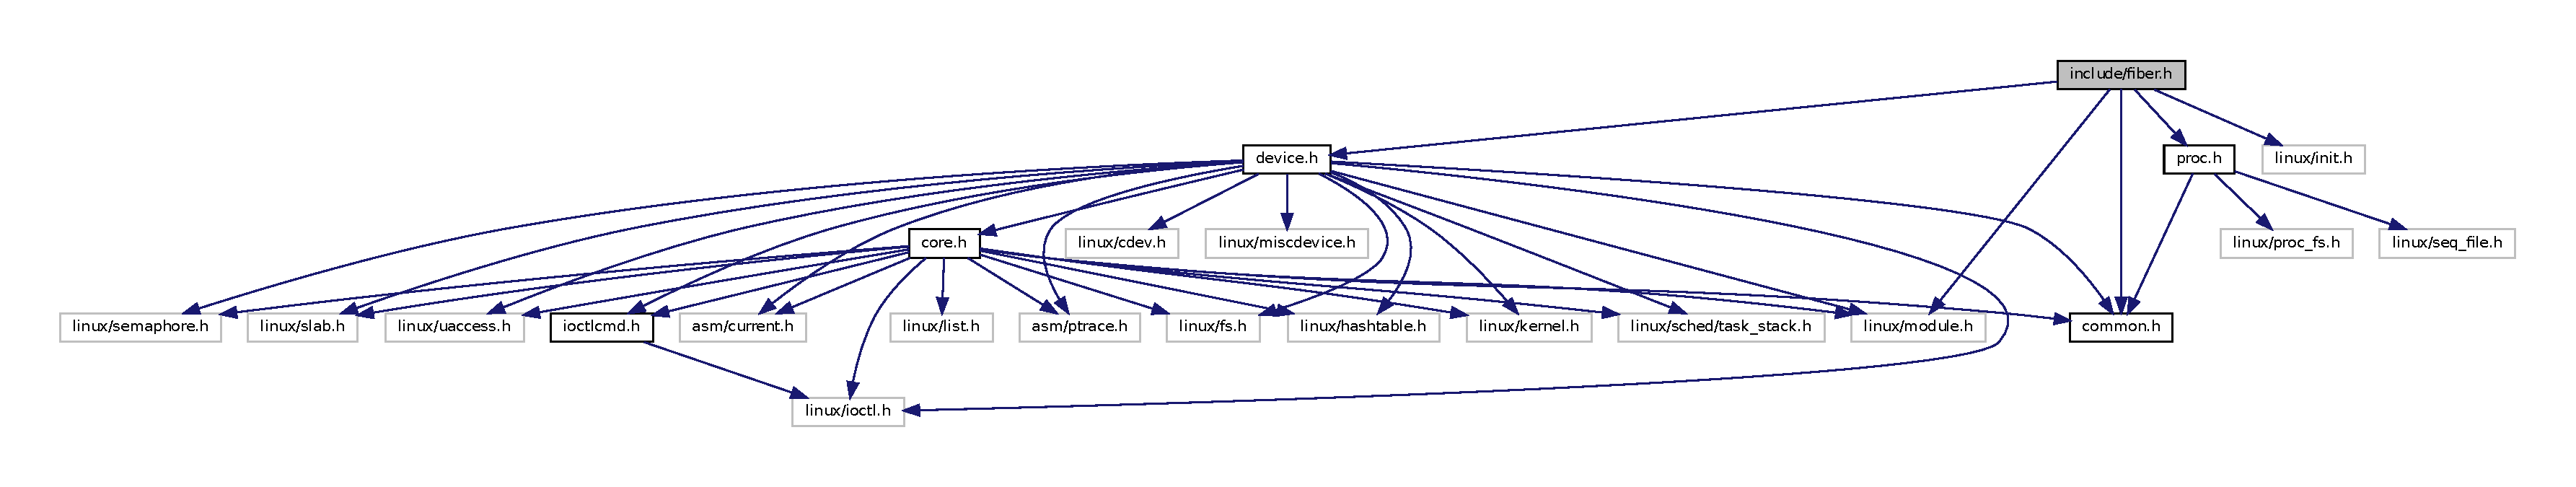
\includegraphics[width=350pt]{fiber_8h__incl}
\end{center}
\end{figure}
This graph shows which files directly or indirectly include this file\+:
\nopagebreak
\begin{figure}[H]
\begin{center}
\leavevmode
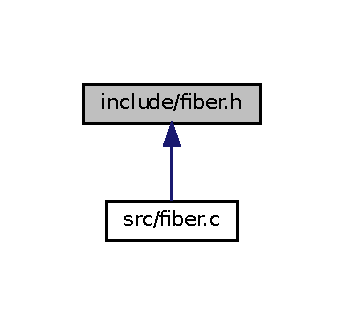
\includegraphics[width=165pt]{fiber_8h__dep__incl}
\end{center}
\end{figure}
\subsection*{Macros}
\begin{DoxyCompactItemize}
\item 
\mbox{\Hypertarget{fiber_8h_a5043e17916c517921959c359078e80b8}\label{fiber_8h_a5043e17916c517921959c359078e80b8}} 
\#define {\bfseries F\+I\+B\+E\+R\+\_\+\+L\+OG}~\char`\"{}\+: F\+I\+B\+E\+R\+: \char`\"{}
\end{DoxyCompactItemize}


\subsection{Detailed Description}
This file contains definitions and macros of the starting point part of the module. 

\begin{DoxyAuthor}{Author}
Gabriele Proietti Mattia \href{mailto:gabry.gabry@hotmail.it}{\tt gabry.\+gabry@hotmail.\+it} 

Alexandru Daniel Tufa \href{mailto:alex.tufa94@gmail.com}{\tt alex.\+tufa94@gmail.\+com} 
\end{DoxyAuthor}
\begin{DoxyDate}{Date}
2018-\/05-\/13 
\end{DoxyDate}

\hypertarget{ioctlcmd_8h}{}\section{include/ioctlcmd.h File Reference}
\label{ioctlcmd_8h}\index{include/ioctlcmd.\+h@{include/ioctlcmd.\+h}}


This file contains definitions of ioctl commands.  


{\ttfamily \#include $<$linux/ioctl.\+h$>$}\newline
Include dependency graph for ioctlcmd.\+h\+:
\nopagebreak
\begin{figure}[H]
\begin{center}
\leavevmode
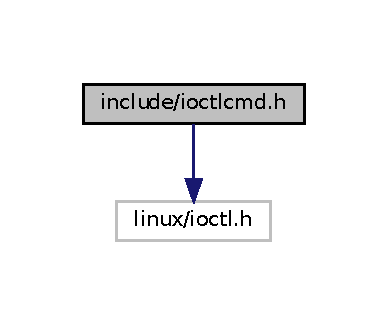
\includegraphics[width=186pt]{ioctlcmd_8h__incl}
\end{center}
\end{figure}
This graph shows which files directly or indirectly include this file\+:
\nopagebreak
\begin{figure}[H]
\begin{center}
\leavevmode
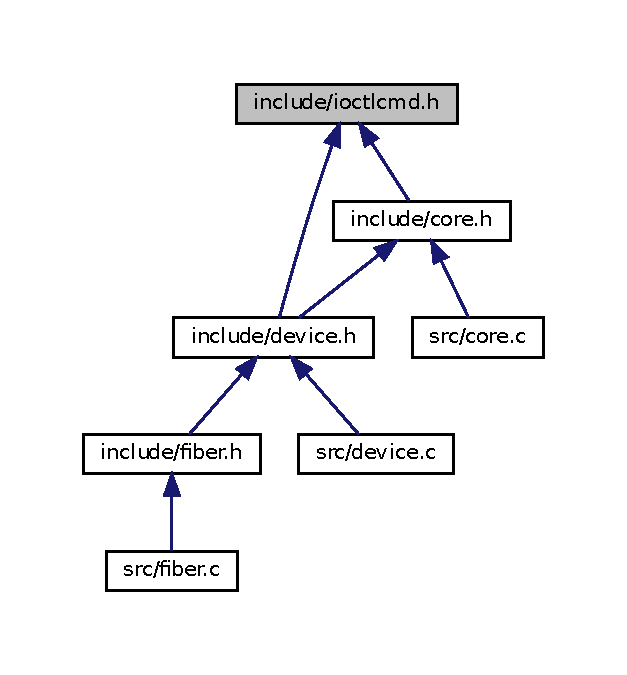
\includegraphics[width=301pt]{ioctlcmd_8h__dep__incl}
\end{center}
\end{figure}
\subsection*{Macros}
\begin{DoxyCompactItemize}
\item 
\mbox{\Hypertarget{ioctlcmd_8h_a3fa8721290c13653f9d838794d7ee261}\label{ioctlcmd_8h_a3fa8721290c13653f9d838794d7ee261}} 
\#define {\bfseries F\+I\+B\+E\+R\+\_\+\+I\+O\+C\+\_\+\+M\+A\+G\+IC}~0x\+F1
\item 
\mbox{\Hypertarget{ioctlcmd_8h_a0fe5046498c1c9c1f58df873802329f8}\label{ioctlcmd_8h_a0fe5046498c1c9c1f58df873802329f8}} 
\#define {\bfseries F\+I\+B\+E\+R\+\_\+\+I\+O\+C\+R\+E\+S\+ET}~\+\_\+\+IO(F\+I\+B\+E\+R\+\_\+\+I\+O\+C\+\_\+\+M\+A\+G\+IC, 0)
\item 
\mbox{\Hypertarget{ioctlcmd_8h_a16f37437f12488e28b159071431a79e5}\label{ioctlcmd_8h_a16f37437f12488e28b159071431a79e5}} 
\#define {\bfseries F\+I\+B\+E\+R\+\_\+\+I\+O\+C\+\_\+\+C\+O\+N\+V\+E\+R\+T\+T\+H\+R\+E\+A\+D\+T\+O\+F\+I\+B\+ER}~\+\_\+\+IO(F\+I\+B\+E\+R\+\_\+\+I\+O\+C\+\_\+\+M\+A\+G\+IC, 1)
\item 
\mbox{\Hypertarget{ioctlcmd_8h_ade67fad05a99e6ec17b0526e5e55eba0}\label{ioctlcmd_8h_ade67fad05a99e6ec17b0526e5e55eba0}} 
\#define {\bfseries F\+I\+B\+E\+R\+\_\+\+I\+O\+C\+\_\+\+C\+R\+E\+A\+T\+E\+F\+I\+B\+ER}~\+\_\+\+I\+OW(F\+I\+B\+E\+R\+\_\+\+I\+O\+C\+\_\+\+M\+A\+G\+IC, 2, int)
\item 
\mbox{\Hypertarget{ioctlcmd_8h_a8c285b2a6378660f8b4b3bd57087655e}\label{ioctlcmd_8h_a8c285b2a6378660f8b4b3bd57087655e}} 
\#define {\bfseries F\+I\+B\+E\+R\+\_\+\+I\+O\+C\+\_\+\+S\+W\+I\+T\+C\+H\+T\+O\+F\+I\+B\+ER}~\+\_\+\+IO(F\+I\+B\+E\+R\+\_\+\+I\+O\+C\+\_\+\+M\+A\+G\+IC, 3)
\item 
\mbox{\Hypertarget{ioctlcmd_8h_a8b452a3bcd354dab866a9951f1e11cfc}\label{ioctlcmd_8h_a8b452a3bcd354dab866a9951f1e11cfc}} 
\#define {\bfseries F\+I\+B\+E\+R\+\_\+\+I\+O\+C\+\_\+\+F\+L\+S\+\_\+\+A\+L\+L\+OC}~\+\_\+\+I\+O\+WR(F\+I\+B\+E\+R\+\_\+\+I\+O\+C\+\_\+\+M\+A\+G\+IC, 4, int)
\item 
\mbox{\Hypertarget{ioctlcmd_8h_a7888c883b97e1cc417ef2437874f22d3}\label{ioctlcmd_8h_a7888c883b97e1cc417ef2437874f22d3}} 
\#define {\bfseries F\+I\+B\+E\+R\+\_\+\+I\+O\+C\+\_\+\+F\+L\+S\+\_\+\+F\+R\+EE}~\+\_\+\+I\+OW(F\+I\+B\+E\+R\+\_\+\+I\+O\+C\+\_\+\+M\+A\+G\+IC, 5, int)
\item 
\mbox{\Hypertarget{ioctlcmd_8h_aca78d5f71cce3383c675f5c7e4ff3b09}\label{ioctlcmd_8h_aca78d5f71cce3383c675f5c7e4ff3b09}} 
\#define {\bfseries F\+I\+B\+E\+R\+\_\+\+I\+O\+C\+\_\+\+F\+L\+S\+\_\+\+G\+ET}~\+\_\+\+I\+OR(F\+I\+B\+E\+R\+\_\+\+I\+O\+C\+\_\+\+M\+A\+G\+IC, 6, int)
\item 
\mbox{\Hypertarget{ioctlcmd_8h_a98785938d1b5f470d3b09e032ecac4ac}\label{ioctlcmd_8h_a98785938d1b5f470d3b09e032ecac4ac}} 
\#define {\bfseries F\+I\+B\+E\+R\+\_\+\+I\+O\+C\+\_\+\+F\+L\+S\+\_\+\+S\+ET}~\+\_\+\+I\+OW(F\+I\+B\+E\+R\+\_\+\+I\+O\+C\+\_\+\+M\+A\+G\+IC, 7, int)
\item 
\mbox{\Hypertarget{ioctlcmd_8h_a0518e8a551a25376f65a60e98189cb70}\label{ioctlcmd_8h_a0518e8a551a25376f65a60e98189cb70}} 
\#define {\bfseries F\+I\+B\+E\+R\+\_\+\+I\+O\+C\+\_\+\+M\+A\+X\+NR}~7
\end{DoxyCompactItemize}


\subsection{Detailed Description}
This file contains definitions of ioctl commands. 

\subsection*{Module operations}

We define the following operations for the module that are mapped with the library (Library -\/$>$ Module)
\begin{DoxyItemize}
\item Convert\+Thread\+To\+Fiber -\/$>$ F\+I\+B\+E\+R\+\_\+\+I\+O\+C\+\_\+\+C\+O\+N\+V\+E\+R\+T\+T\+H\+R\+E\+A\+D\+T\+O\+F\+I\+B\+ER
\item Create\+Fiber -\/$>$ F\+I\+B\+E\+R\+\_\+\+I\+O\+C\+\_\+\+C\+R\+E\+A\+T\+E\+F\+I\+B\+ER
\item Switch\+To\+Fiber -\/$>$ F\+I\+B\+E\+R\+\_\+\+I\+O\+C\+\_\+\+S\+W\+I\+T\+C\+H\+T\+O\+F\+I\+B\+ER
\item Fls\+Alloc -\/$>$ F\+L\+S\+\_\+\+A\+L\+L\+OC
\item Fls\+Free -\/$>$ F\+L\+S\+\_\+\+F\+R\+EE
\item Fls\+Get\+Value -\/$>$ F\+L\+S\+\_\+\+G\+ET
\item Fls\+Set\+Value -\/$>$ F\+L\+S\+\_\+\+S\+ET
\end{DoxyItemize}

\begin{DoxyAuthor}{Author}
Gabriele Proietti Mattia \href{mailto:gabry.gabry@hotmail.it}{\tt gabry.\+gabry@hotmail.\+it} 

Alexandru Daniel Tufa \href{mailto:alex.tufa94@gmail.com}{\tt alex.\+tufa94@gmail.\+com} 
\end{DoxyAuthor}
\begin{DoxyDate}{Date}
2018-\/05-\/07 
\end{DoxyDate}

\hypertarget{proc_8h}{}\section{include/proc.h File Reference}
\label{proc_8h}\index{include/proc.\+h@{include/proc.\+h}}


This file contains definitions and macros for the {\itshape proc} part of the module.  


{\ttfamily \#include \char`\"{}common.\+h\char`\"{}}\newline
{\ttfamily \#include $<$linux/proc\+\_\+fs.\+h$>$}\newline
{\ttfamily \#include $<$linux/seq\+\_\+file.\+h$>$}\newline
Include dependency graph for proc.\+h\+:
\nopagebreak
\begin{figure}[H]
\begin{center}
\leavevmode
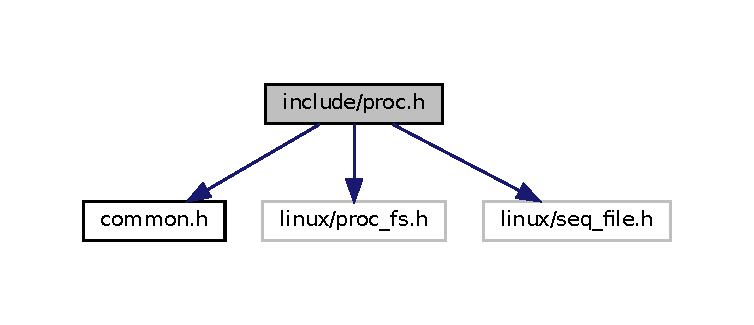
\includegraphics[width=350pt]{proc_8h__incl}
\end{center}
\end{figure}
This graph shows which files directly or indirectly include this file\+:
\nopagebreak
\begin{figure}[H]
\begin{center}
\leavevmode
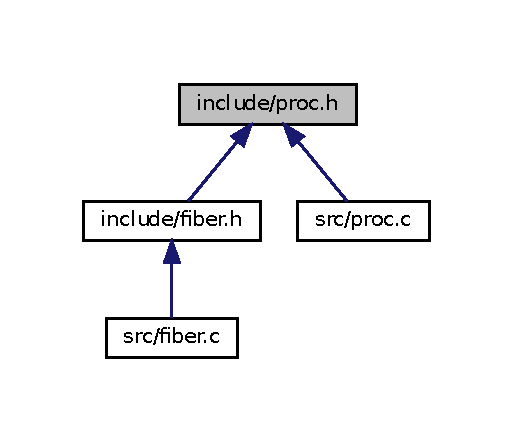
\includegraphics[width=246pt]{proc_8h__dep__incl}
\end{center}
\end{figure}
\subsection*{Macros}
\begin{DoxyCompactItemize}
\item 
\mbox{\Hypertarget{proc_8h_a91eee23c506ccb0b8530e45a3a78a0b5}\label{proc_8h_a91eee23c506ccb0b8530e45a3a78a0b5}} 
\#define {\bfseries P\+R\+O\+C\+\_\+\+L\+OG}~\char`\"{}\+: P\+R\+O\+C\+: \char`\"{}
\item 
\mbox{\Hypertarget{proc_8h_a8c811fa2b4410338baac74a1e6f8db98}\label{proc_8h_a8c811fa2b4410338baac74a1e6f8db98}} 
\#define {\bfseries P\+R\+O\+C\+\_\+\+F\+O\+L\+D\+ER}~\char`\"{}fibers\char`\"{}
\item 
\mbox{\Hypertarget{proc_8h_a8e2554ffb48c1fb5167a9f61045df1f2}\label{proc_8h_a8e2554ffb48c1fb5167a9f61045df1f2}} 
\#define {\bfseries P\+R\+O\+C\+\_\+\+E\+N\+T\+RY}~\char`\"{}fiber\char`\"{}
\end{DoxyCompactItemize}
\subsection*{Functions}
\begin{DoxyCompactItemize}
\item 
int \mbox{\hyperlink{proc_8h_ac259d1fab55f793f322af5233653b7a3}{init\+\_\+proc}} (void)
\begin{DoxyCompactList}\small\item\em Init here all the proc files for the module Inspired by \href{https://static.lwn.net/images/pdf/LDD3/ch04.pdf}{\tt https\+://static.\+lwn.\+net/images/pdf/\+L\+D\+D3/ch04.\+pdf} and updated to new standard. \end{DoxyCompactList}\item 
\mbox{\Hypertarget{proc_8h_abfed4d9c489643f848aa94cb5147df5d}\label{proc_8h_abfed4d9c489643f848aa94cb5147df5d}} 
void \mbox{\hyperlink{proc_8h_abfed4d9c489643f848aa94cb5147df5d}{destroy\+\_\+proc}} (void)
\begin{DoxyCompactList}\small\item\em Destroy all the proc files. \end{DoxyCompactList}\end{DoxyCompactItemize}


\subsection{Detailed Description}
This file contains definitions and macros for the {\itshape proc} part of the module. 

\begin{DoxyAuthor}{Author}
Gabriele Proietti Mattia \href{mailto:gabry.gabry@hotmail.it}{\tt gabry.\+gabry@hotmail.\+it} 

Alexandru Daniel Tufa \href{mailto:alex.tufa94@gmail.com}{\tt alex.\+tufa94@gmail.\+com} 
\end{DoxyAuthor}
\begin{DoxyDate}{Date}
2018-\/05-\/13 
\end{DoxyDate}


\subsection{Function Documentation}
\mbox{\Hypertarget{proc_8h_ac259d1fab55f793f322af5233653b7a3}\label{proc_8h_ac259d1fab55f793f322af5233653b7a3}} 
\index{proc.\+h@{proc.\+h}!init\+\_\+proc@{init\+\_\+proc}}
\index{init\+\_\+proc@{init\+\_\+proc}!proc.\+h@{proc.\+h}}
\subsubsection{\texorpdfstring{init\+\_\+proc()}{init\_proc()}}
{\footnotesize\ttfamily int init\+\_\+proc (\begin{DoxyParamCaption}\item[{void}]{ }\end{DoxyParamCaption})}



Init here all the proc files for the module Inspired by \href{https://static.lwn.net/images/pdf/LDD3/ch04.pdf}{\tt https\+://static.\+lwn.\+net/images/pdf/\+L\+D\+D3/ch04.\+pdf} and updated to new standard. 

\begin{DoxyReturn}{Returns}
int 
\end{DoxyReturn}

\hypertarget{core_8c}{}\section{src/core.c File Reference}
\label{core_8c}\index{src/core.\+c@{src/core.\+c}}


This file contains the implementation of all the core functions of the module.  


{\ttfamily \#include \char`\"{}core.\+h\char`\"{}}\newline
Include dependency graph for core.\+c\+:
\nopagebreak
\begin{figure}[H]
\begin{center}
\leavevmode
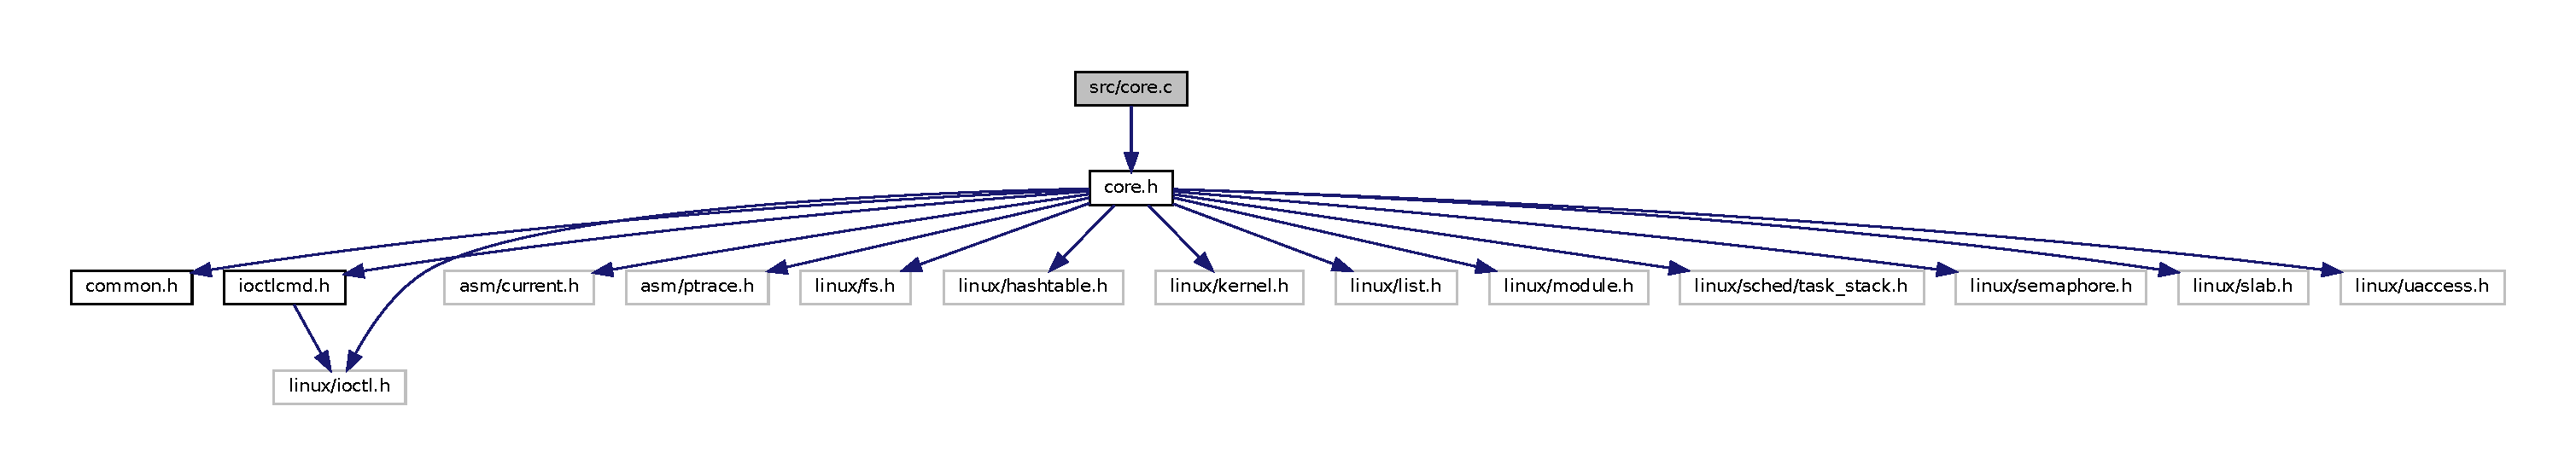
\includegraphics[width=350pt]{core_8c__incl}
\end{center}
\end{figure}
\subsection*{Functions}
\begin{DoxyCompactItemize}
\item 
int \mbox{\hyperlink{core_8c_a0901eb890c674d9f7f5e97316fc67a2c}{convert\+\_\+thread\+\_\+to\+\_\+fiber}} ()
\begin{DoxyCompactList}\small\item\em Convert the current thread to a fiber. \end{DoxyCompactList}\end{DoxyCompactItemize}


\subsection{Detailed Description}
This file contains the implementation of all the core functions of the module. 

\begin{DoxyAuthor}{Author}
Gabriele Proietti Mattia \href{mailto:gabry.gabry@hotmail.it}{\tt gabry.\+gabry@hotmail.\+it} 

Alexandru Daniel Tufa \href{mailto:alex.tufa94@gmail.com}{\tt alex.\+tufa94@gmail.\+com} 
\end{DoxyAuthor}
\begin{DoxyDate}{Date}
2018-\/05-\/13 
\end{DoxyDate}


\subsection{Function Documentation}
\mbox{\Hypertarget{core_8c_a0901eb890c674d9f7f5e97316fc67a2c}\label{core_8c_a0901eb890c674d9f7f5e97316fc67a2c}} 
\index{core.\+c@{core.\+c}!convert\+\_\+thread\+\_\+to\+\_\+fiber@{convert\+\_\+thread\+\_\+to\+\_\+fiber}}
\index{convert\+\_\+thread\+\_\+to\+\_\+fiber@{convert\+\_\+thread\+\_\+to\+\_\+fiber}!core.\+c@{core.\+c}}
\subsubsection{\texorpdfstring{convert\+\_\+thread\+\_\+to\+\_\+fiber()}{convert\_thread\_to\_fiber()}}
{\footnotesize\ttfamily int convert\+\_\+thread\+\_\+to\+\_\+fiber (\begin{DoxyParamCaption}\item[{void}]{ }\end{DoxyParamCaption})}



Convert the current thread to a fiber. 

\subsection*{Implementation}

When a thread is converted to a fiber several task are performed. First of all, if the process never created a fiber, it must become {\bfseries fiber-\/enabled}, this means that we have to instantiate a \mbox{\hyperlink{structfibered__process}{fibered\+\_\+process}} element in the \mbox{\hyperlink{structfibered__processes__list}{fibered\+\_\+processes\+\_\+list}} variable. Then we have to instantiate a \mbox{\hyperlink{structfiber}{fiber}} element in the \mbox{\hyperlink{structfibers__list}{fibers\+\_\+list}} field of the \mbox{\hyperlink{structfibered__process}{fibered\+\_\+process}} element of the list.

\begin{DoxyReturn}{Returns}
int 0 if everything ok, otherwise an error listed in \mbox{\hyperlink{ioctlcmd_8h}{ioctlcmd.\+h}} 
\end{DoxyReturn}

\hypertarget{device_8c}{}\section{src/device.c File Reference}
\label{device_8c}\index{src/device.\+c@{src/device.\+c}}


This file contains the implementation of the char device.  


{\ttfamily \#include \char`\"{}device.\+h\char`\"{}}\newline
Include dependency graph for device.\+c\+:
\nopagebreak
\begin{figure}[H]
\begin{center}
\leavevmode
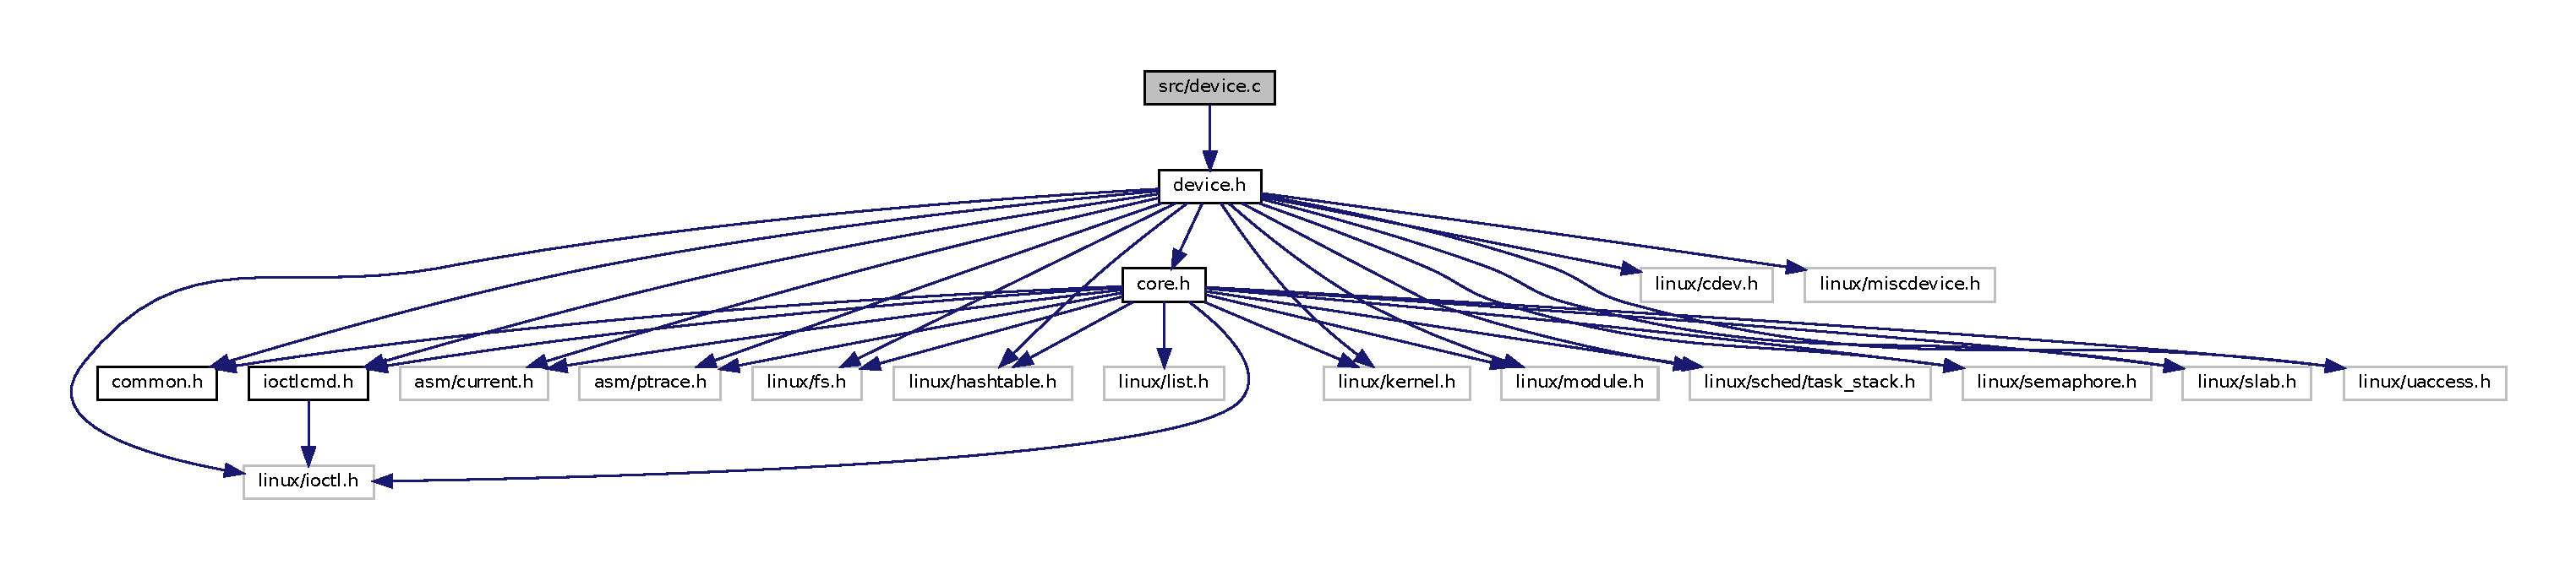
\includegraphics[width=350pt]{device_8c__incl}
\end{center}
\end{figure}
\subsection*{Functions}
\begin{DoxyCompactItemize}
\item 
int \mbox{\hyperlink{device_8c_a88bd4adb20dc9040ae78f5b4036b61ab}{init\+\_\+device}} (void)
\begin{DoxyCompactList}\small\item\em Init the device inspired by \href{https://www.linuxjournal.com/article/2920}{\tt https\+://www.\+linuxjournal.\+com/article/2920}. \end{DoxyCompactList}\item 
\mbox{\Hypertarget{device_8c_a80ad9d4cfc87c34e428952a2d24b73e5}\label{device_8c_a80ad9d4cfc87c34e428952a2d24b73e5}} 
void \mbox{\hyperlink{device_8c_a80ad9d4cfc87c34e428952a2d24b73e5}{destroy\+\_\+device}} (void)
\begin{DoxyCompactList}\small\item\em Destroy the device. \end{DoxyCompactList}\end{DoxyCompactItemize}


\subsection{Detailed Description}
This file contains the implementation of the char device. 

\begin{DoxyAuthor}{Author}
Gabriele Proietti Mattia \href{mailto:gabry.gabry@hotmail.it}{\tt gabry.\+gabry@hotmail.\+it} 

Alexandru Daniel Tufa \href{mailto:alex.tufa94@gmail.com}{\tt alex.\+tufa94@gmail.\+com} 
\end{DoxyAuthor}
\begin{DoxyDate}{Date}
2018-\/05-\/06 
\end{DoxyDate}


\subsection{Function Documentation}
\mbox{\Hypertarget{device_8c_a88bd4adb20dc9040ae78f5b4036b61ab}\label{device_8c_a88bd4adb20dc9040ae78f5b4036b61ab}} 
\index{device.\+c@{device.\+c}!init\+\_\+device@{init\+\_\+device}}
\index{init\+\_\+device@{init\+\_\+device}!device.\+c@{device.\+c}}
\subsubsection{\texorpdfstring{init\+\_\+device()}{init\_device()}}
{\footnotesize\ttfamily int init\+\_\+device (\begin{DoxyParamCaption}\item[{void}]{ }\end{DoxyParamCaption})}



Init the device inspired by \href{https://www.linuxjournal.com/article/2920}{\tt https\+://www.\+linuxjournal.\+com/article/2920}. 

\begin{DoxyReturn}{Returns}
int 
\end{DoxyReturn}

\hypertarget{fiber_8c}{}\section{src/fiber.c File Reference}
\label{fiber_8c}\index{src/fiber.\+c@{src/fiber.\+c}}


This file is the starting point of the module.  


{\ttfamily \#include \char`\"{}fiber.\+h\char`\"{}}\newline
Include dependency graph for fiber.\+c\+:
\nopagebreak
\begin{figure}[H]
\begin{center}
\leavevmode
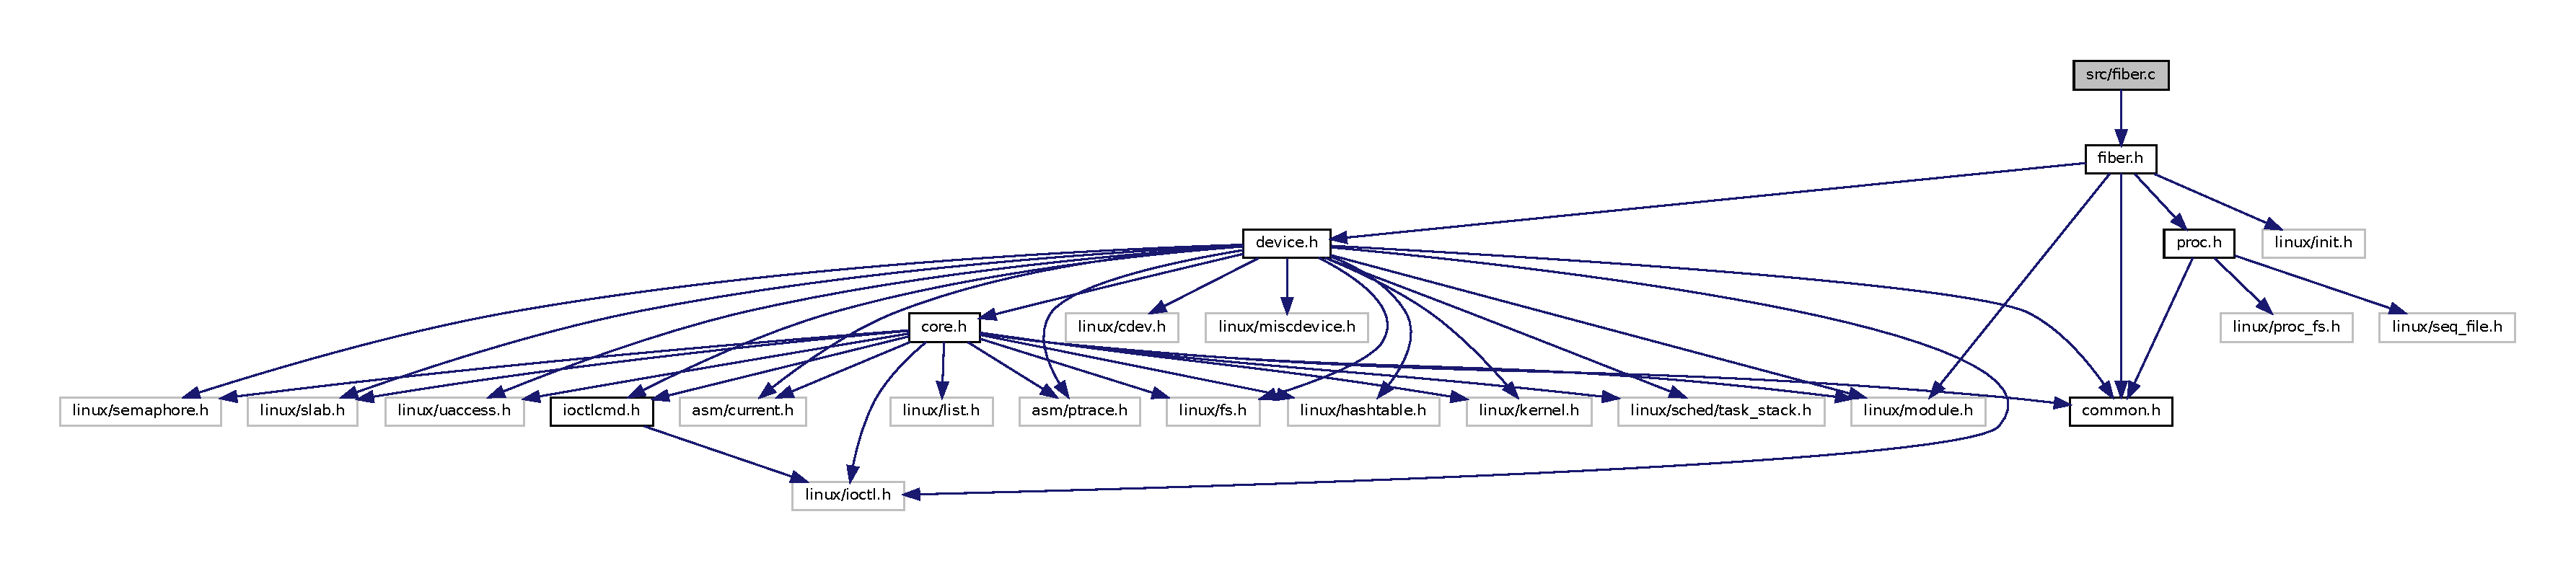
\includegraphics[width=350pt]{fiber_8c__incl}
\end{center}
\end{figure}
\subsection*{Functions}
\begin{DoxyCompactItemize}
\item 
\mbox{\Hypertarget{fiber_8c_ad94b36675e7eb067ea3ce6ff9e244a44}\label{fiber_8c_ad94b36675e7eb067ea3ce6ff9e244a44}} 
{\bfseries M\+O\+D\+U\+L\+E\+\_\+\+L\+I\+C\+E\+N\+SE} (\char`\"{}G\+PL\char`\"{})
\item 
\mbox{\Hypertarget{fiber_8c_a91c7dd13520e5d6d04bcd1f29448e10d}\label{fiber_8c_a91c7dd13520e5d6d04bcd1f29448e10d}} 
{\bfseries module\+\_\+init} (init\+\_\+fiber)
\item 
\mbox{\Hypertarget{fiber_8c_aaac60d4f12bc7ddbd5d64cc095f060bc}\label{fiber_8c_aaac60d4f12bc7ddbd5d64cc095f060bc}} 
{\bfseries module\+\_\+exit} (destroy\+\_\+fiber)
\end{DoxyCompactItemize}


\subsection{Detailed Description}
This file is the starting point of the module. 

\begin{DoxyAuthor}{Author}
Gabriele Proietti Mattia \href{mailto:gabry.gabry@hotmail.it}{\tt gabry.\+gabry@hotmail.\+it} 

Alexandru Daniel Tufa \href{mailto:alex.tufa94@gmail.com}{\tt alex.\+tufa94@gmail.\+com} 
\end{DoxyAuthor}
\begin{DoxyDate}{Date}
2018-\/05-\/06 
\end{DoxyDate}

\hypertarget{proc_8c}{}\section{src/proc.c File Reference}
\label{proc_8c}\index{src/proc.\+c@{src/proc.\+c}}


This file contains the implementation of the /proc fs files.  


{\ttfamily \#include \char`\"{}proc.\+h\char`\"{}}\newline
Include dependency graph for proc.\+c\+:
\nopagebreak
\begin{figure}[H]
\begin{center}
\leavevmode
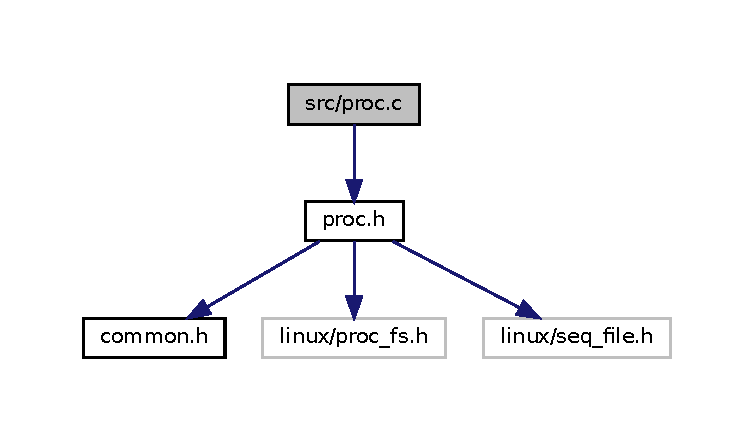
\includegraphics[width=350pt]{proc_8c__incl}
\end{center}
\end{figure}
\subsection*{Functions}
\begin{DoxyCompactItemize}
\item 
int \mbox{\hyperlink{proc_8c_ac1cb67a3c8f09a371d771862ebc2f578}{init\+\_\+proc}} ()
\begin{DoxyCompactList}\small\item\em Init here all the proc files for the module Inspired by \href{https://static.lwn.net/images/pdf/LDD3/ch04.pdf}{\tt https\+://static.\+lwn.\+net/images/pdf/\+L\+D\+D3/ch04.\+pdf} and updated to new standard. \end{DoxyCompactList}\item 
\mbox{\Hypertarget{proc_8c_adc42369799f038365080b4111bbd6b52}\label{proc_8c_adc42369799f038365080b4111bbd6b52}} 
void \mbox{\hyperlink{proc_8c_adc42369799f038365080b4111bbd6b52}{destroy\+\_\+proc}} ()
\begin{DoxyCompactList}\small\item\em Destroy all the proc files. \end{DoxyCompactList}\end{DoxyCompactItemize}


\subsection{Detailed Description}
This file contains the implementation of the /proc fs files. 

\begin{DoxyAuthor}{Author}
Gabriele Proietti Mattia \href{mailto:gabry.gabry@hotmail.it}{\tt gabry.\+gabry@hotmail.\+it} 

Alexandru Daniel Tufa \href{mailto:alex.tufa94@gmail.com}{\tt alex.\+tufa94@gmail.\+com} 
\end{DoxyAuthor}
\begin{DoxyDate}{Date}
2018-\/05-\/06 
\end{DoxyDate}


\subsection{Function Documentation}
\mbox{\Hypertarget{proc_8c_ac1cb67a3c8f09a371d771862ebc2f578}\label{proc_8c_ac1cb67a3c8f09a371d771862ebc2f578}} 
\index{proc.\+c@{proc.\+c}!init\+\_\+proc@{init\+\_\+proc}}
\index{init\+\_\+proc@{init\+\_\+proc}!proc.\+c@{proc.\+c}}
\subsubsection{\texorpdfstring{init\+\_\+proc()}{init\_proc()}}
{\footnotesize\ttfamily int init\+\_\+proc (\begin{DoxyParamCaption}\item[{void}]{ }\end{DoxyParamCaption})}



Init here all the proc files for the module Inspired by \href{https://static.lwn.net/images/pdf/LDD3/ch04.pdf}{\tt https\+://static.\+lwn.\+net/images/pdf/\+L\+D\+D3/ch04.\+pdf} and updated to new standard. 

\begin{DoxyReturn}{Returns}
int 
\end{DoxyReturn}

%--- End generated contents ---

% Index
\backmatter
\newpage
\phantomsection
\clearemptydoublepage
\addcontentsline{toc}{chapter}{Index}
\printindex

\end{document}
